
\documentclass[10pt]{beamer}

\usetheme{metropolis}
\usepackage{appendixnumberbeamer}
\usepackage{graphicx}
\usepackage{animate}
\usepackage{hyperref}
\usepackage{booktabs}
\usepackage[scale=2]{ccicons}
\usepackage{tikz}
\usetikzlibrary{positioning}
\usetikzlibrary{shapes,snakes}
\usepackage{pgfplots}
\usepgfplotslibrary{dateplot}
\usepackage{subcaption}
\usepackage{xspace}
\newcommand{\themename}{\textbf{\textsc{metropolis}}\xspace}
\title{Low-level controller for non-holonomic omnidirectional mobile robot}
\date{\today}
\author{Lingyuan Yang}
\institute{Technische Universität Berlin\\ABB Corporate Research}


\tikzset{
    wheelFrame/.pic={
		\draw[gray, very thick] (-0.8,-0.1) rectangle (0.8,0.1);
		\filldraw [gray] (0,0) circle (1pt);
		\draw[->] (0,0) -- (1,0) node[anchor=north west] {$x^{w#1}$};
		\draw[->] (0,0) -- (0,1) node[anchor=north west] {$y^{w#1}$}; 
	}
}
\tikzset{
    wheel/.pic={
		\draw[gray, very thick] (-0.8,-0.1) rectangle (0.8,0.1);
		\filldraw [gray] (0,0) circle (1pt);
	}
}


\tikzset{
    platform/.pic={
		\filldraw [gray] (0,0) circle (2pt);
			\draw[thick,->] (0,0) -- (5,0) node[anchor=north west] {$x^b$};
			\draw[thick,->] (0,0) -- (0,5) node[anchor=south east] {$y^b$};
			\draw[thick,->] (0.75,0) arc (0:90:0.75) node[anchor=south west] {$\theta^b$};
			\draw[black, thick] (-3,-3) rectangle (3,3);
	}
}










\begin{document}

\maketitle

\begin{frame}{Table of contents}
  \setbeamertemplate{section in toc}[sections numbered]
  \tableofcontents[hideallsubsections]
\end{frame}

\section{Introduction}
%%%%%%%%%%%%%%%%%%%%%%%%%%%%%%%%%%%%%%%%%%%%%%%%%%%%%%%%%%%%%%%%%
\begin{frame}{Mobile Platform}
    \begin{figure}
        \centering
        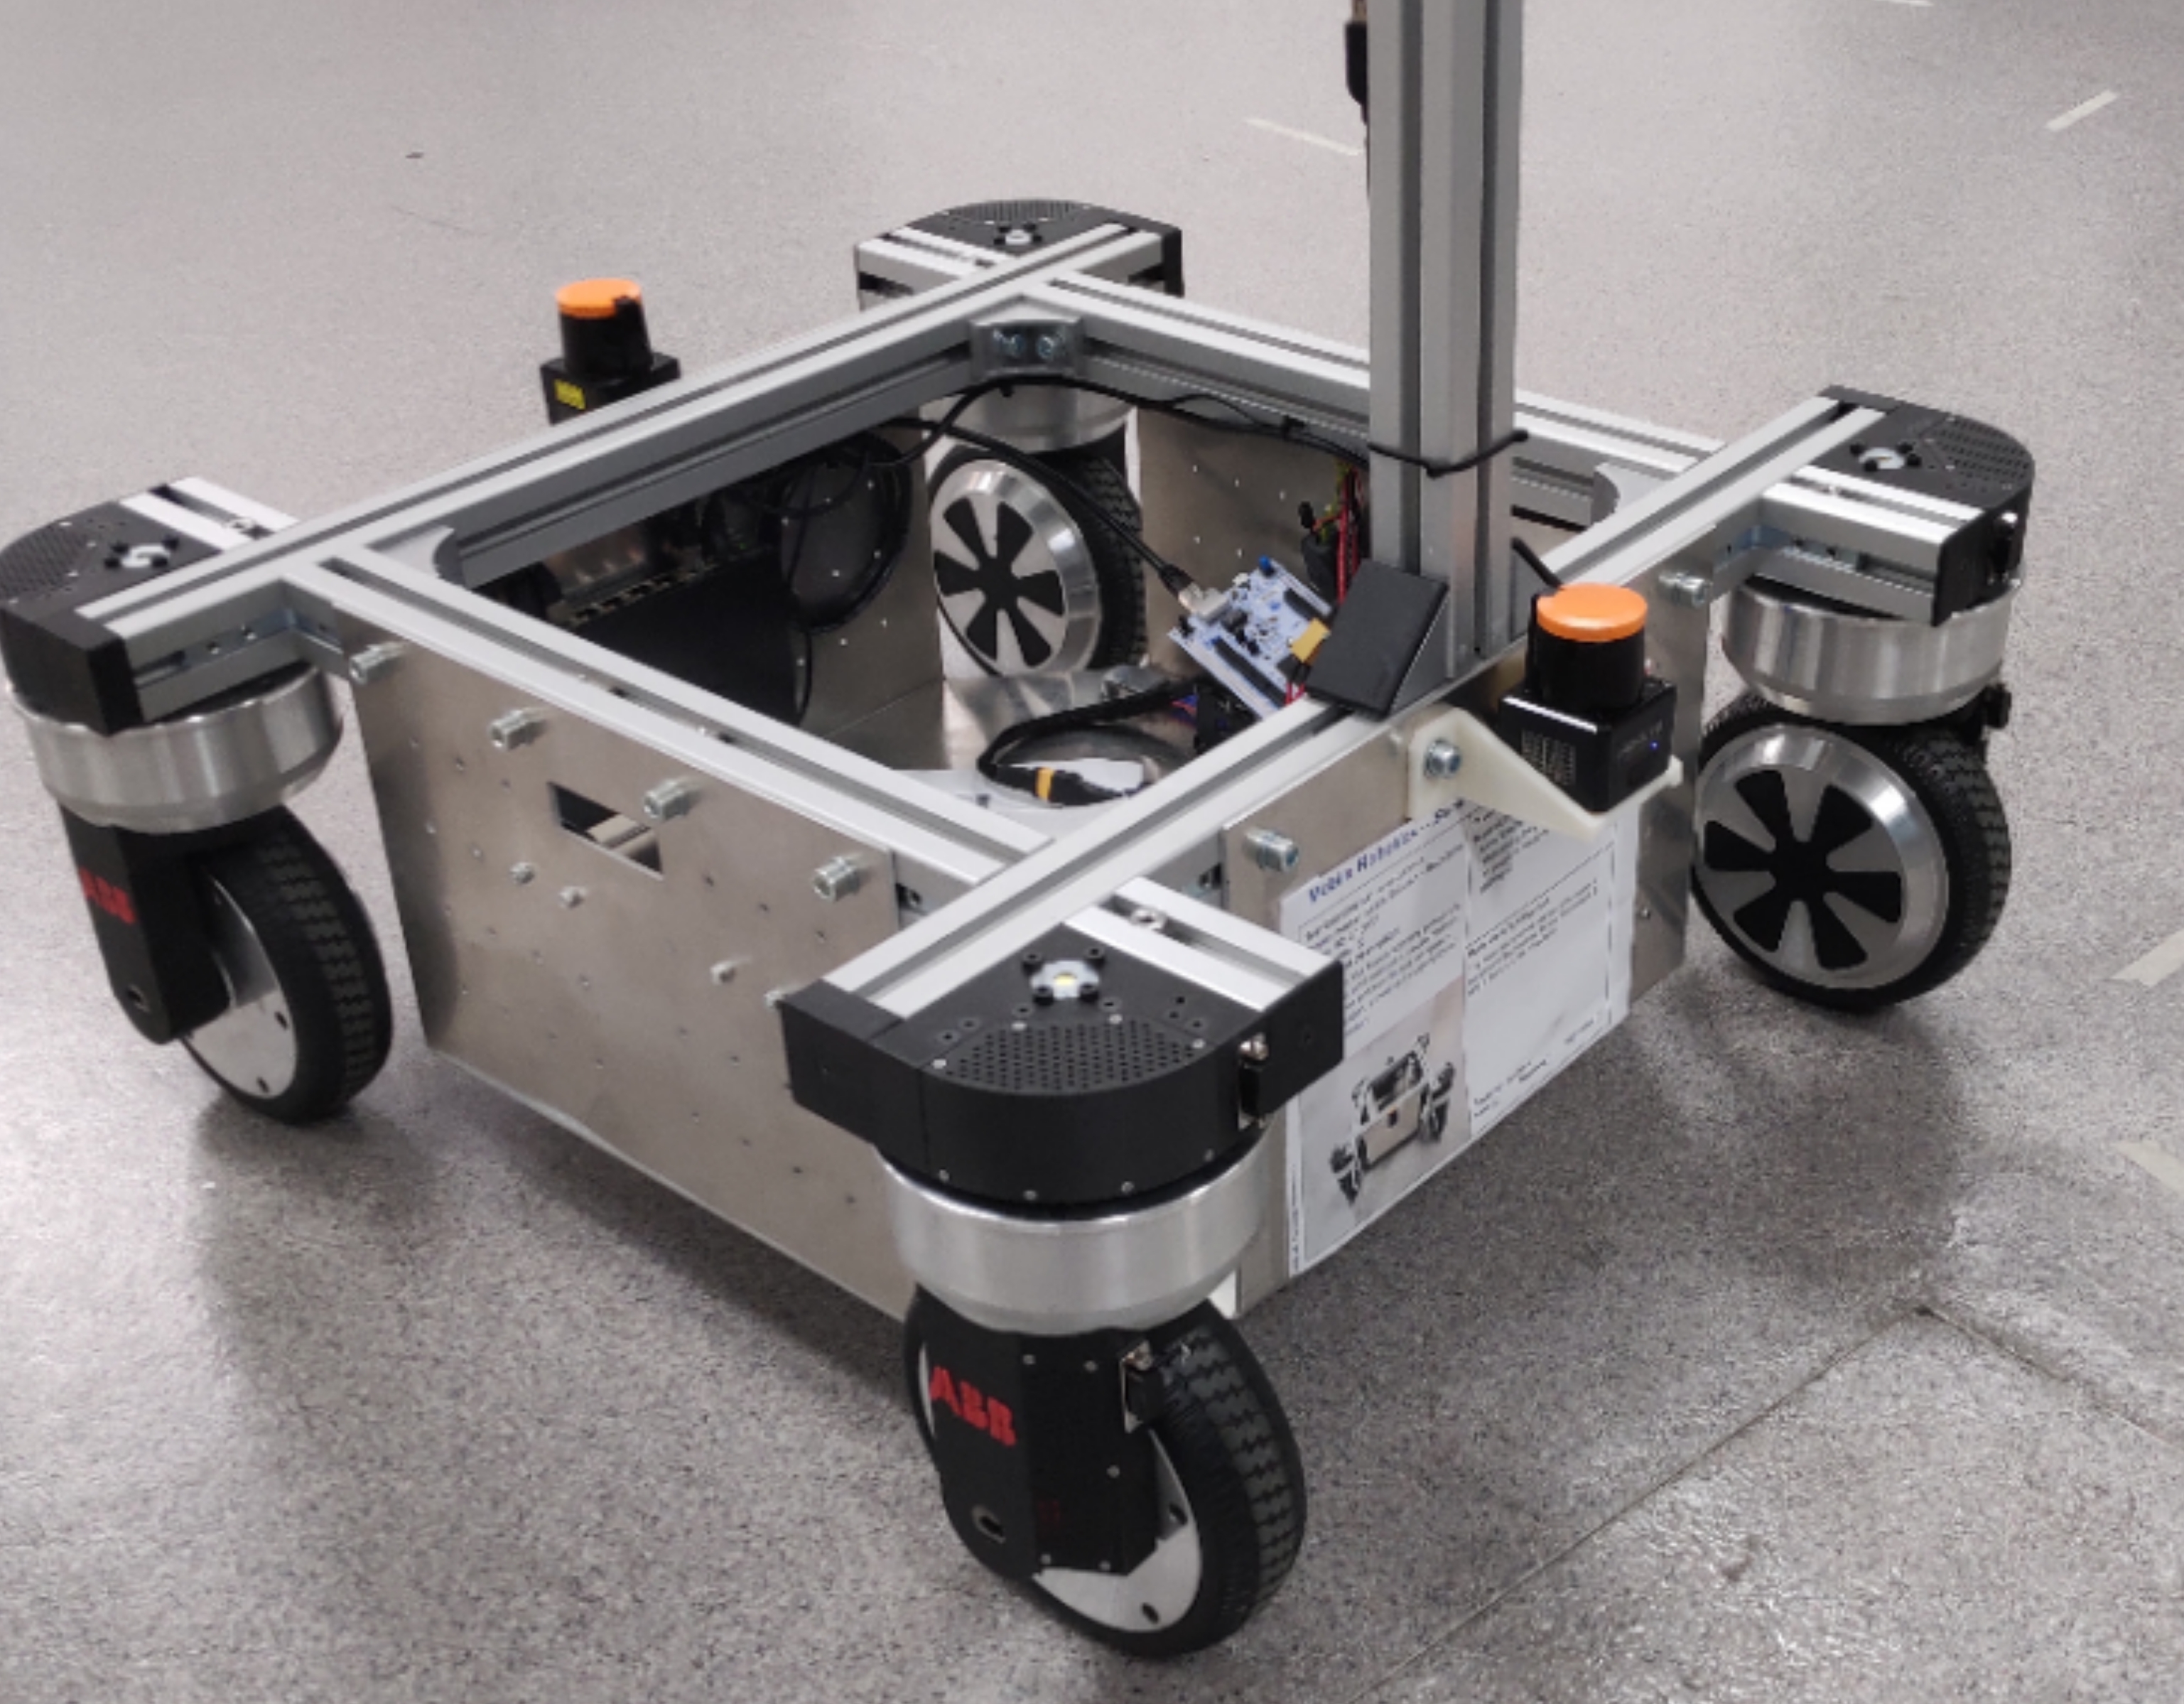
\includegraphics[width=\textwidth]{Figure/mobilePlatform.jpg}
        \caption{}
        \label{fig:mobilePlatform}
    \end{figure}
\end{frame}
%%%%%%%%%%%%%%%%%%%%%%%%%%%%%%%%%%%%%%%%%%%%%%%%%%%%%%%%%%%%%%%%%
\begin{frame}{Non-holonomic omnidirectional mobile robot}
    	\begin{alertblock}{Non-holonomic}
		\textbf{Controlable DoF less than DoF} The mobile robot have 3 DoF $x,y,\theta$. But it cannot do arbitrary velocity instantaneously. The wheels needs to orient to a certain position to achieve a certain velocity.\\ Eg. Move a shopping cart sideways.
		\begin{figure}
		    \centering
		    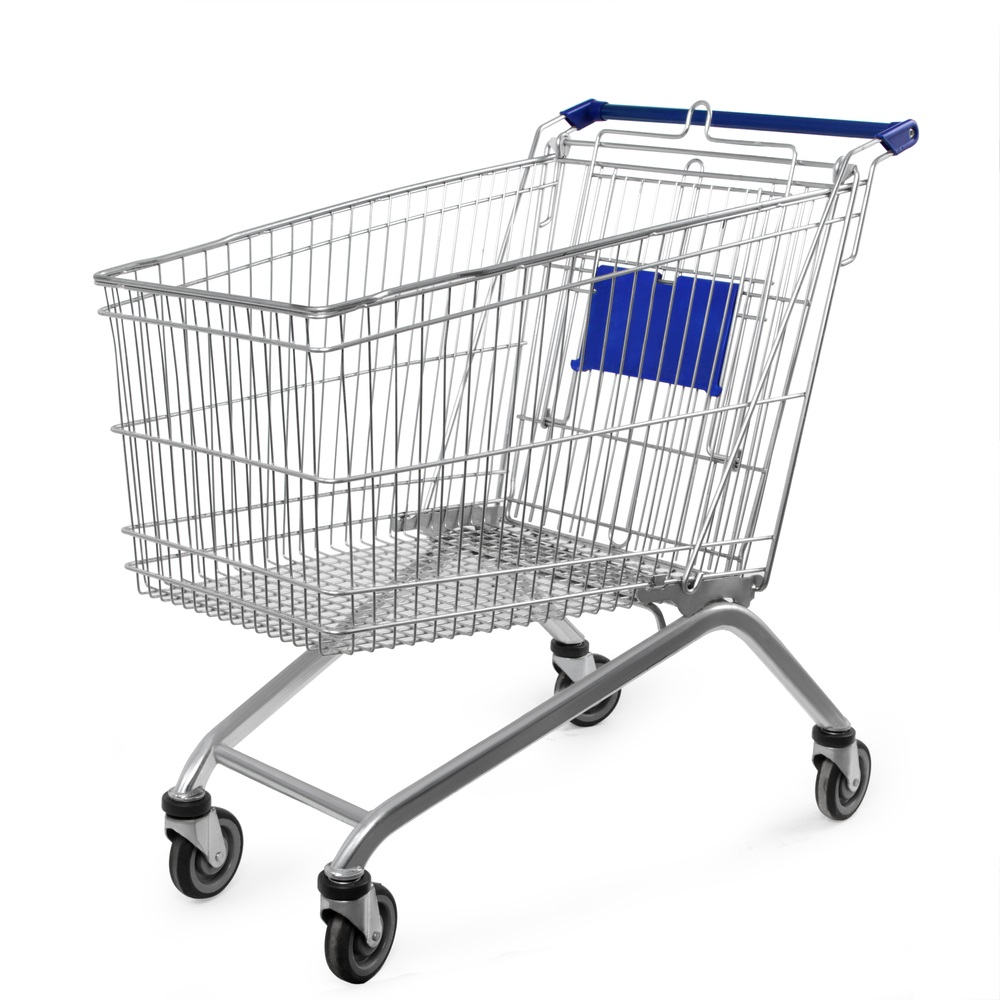
\includegraphics[width=0.4\textwidth]{Figure/shoppingcartwalmart.jpg}
		    \caption{Caption}
		    \label{fig:my_label}
		\end{figure}
	\end{alertblock}
\end{frame}
%%%%%%%%%%%%%%%%%%%%%%%%%%%%%%%%%%%%%%%%%%%%%%%%%%%%%%%%%%%%%%%%%
\begin{frame}{Non-holonomic omnidirectional mobile robot}
    	\begin{alertblock}{omnidirectional}
		The mobile robot can acheive any task space velocity $\dot{x},\dot{y},\dot{\theta}$ if properly initialized.
		Eg. turn all the wheels 90 degree to move sideways.
	\end{alertblock}
\end{frame}
%%%%%%%%%%%%%%%%%%%%%%%%%%%%%%%%%%%%%%%%%%%%%%%%%%%%%%%%%%%%%%%%%


%%%%%%%%%%%%%%%%%%%%%%%%%%%%%%%%%%%%%%%%%%%%%%%%%%%%%%%%%%%%%%%%%

\begin{frame}{Counterparties}
    \begin{itemize}
        \item Differential drive - not flexibel
        \item Swedish wheel - not robust
    \end{itemize}
    \begin{columns}
      \column{0.5\textwidth}
      \begin{figure}
          \centering
          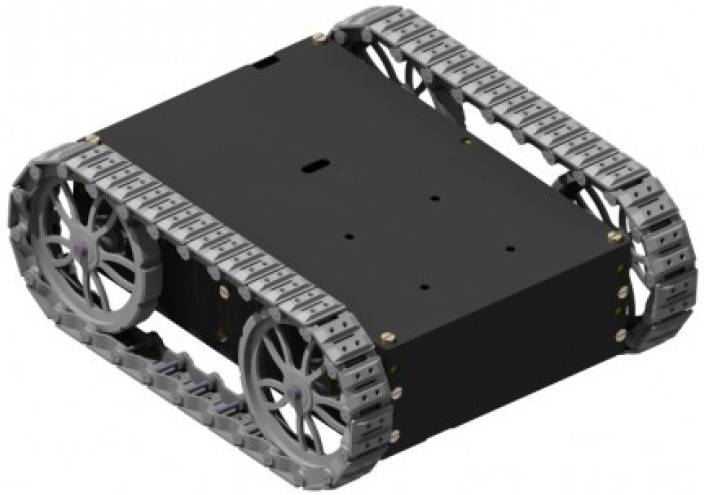
\includegraphics[width=\textwidth]{Figure/tank.jpeg}
          \caption{Differential drive}
          \label{fig:my_label}
      \end{figure}
      
      \column{0.5\textwidth}
      \begin{figure}
          \centering
          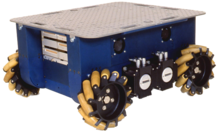
\includegraphics[width=\textwidth]{Figure/swedish.png}
          \caption{Swedish wheel}
          \label{fig:my_label}
      \end{figure}
    \end{columns}
\end{frame}
%%%%%%%%%%%%%%%%%%%%%%%%%%%%%%%%%%%%%%%%%%%%%%%%%%%%%%%%%%%%%%%%%

\section{Kinematics}

%%%%%%%%%%%%%%%%%%%%%%%%%%%%%%%%%%%%%%%%%%%%%%%%%%%%%%%%%%%%%%%%%
\begin{frame}{Kinematics Constraints}
    Kinematics constrain the movement of components of a mechanical system.
    Fundamental for our controller, mapping the task space velocity $\dot{\xi}=[\dot{x},\dot{y},\dot{\theta}]$ to corresponding joint configuration $\beta,\dot{\beta},\dot{\phi}$.
    \begin{equation}
        \begin{split}
            [\beta,\dot{\beta},\dot{\phi}]^T=Kinematics(\dot{\xi},\ddot{\xi})
        \end{split}
    \end{equation}

            \begin{figure}
                \centering

                \begin{subfigure}[t]{0.4\textwidth}
                    \centering
                    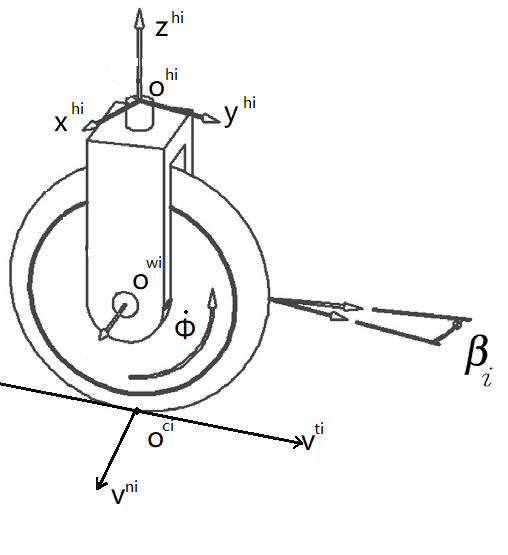
\includegraphics[width=0.8\linewidth]{Figure/wheel.png}
                    \caption{Joint configuration}
                    \label{fig:sub1}
                \end{subfigure}\hskip 1em%
                \begin{subfigure}[t]{0.5\textwidth}
                    \centering
                    \resizebox{5cm}{!}
                    {
		                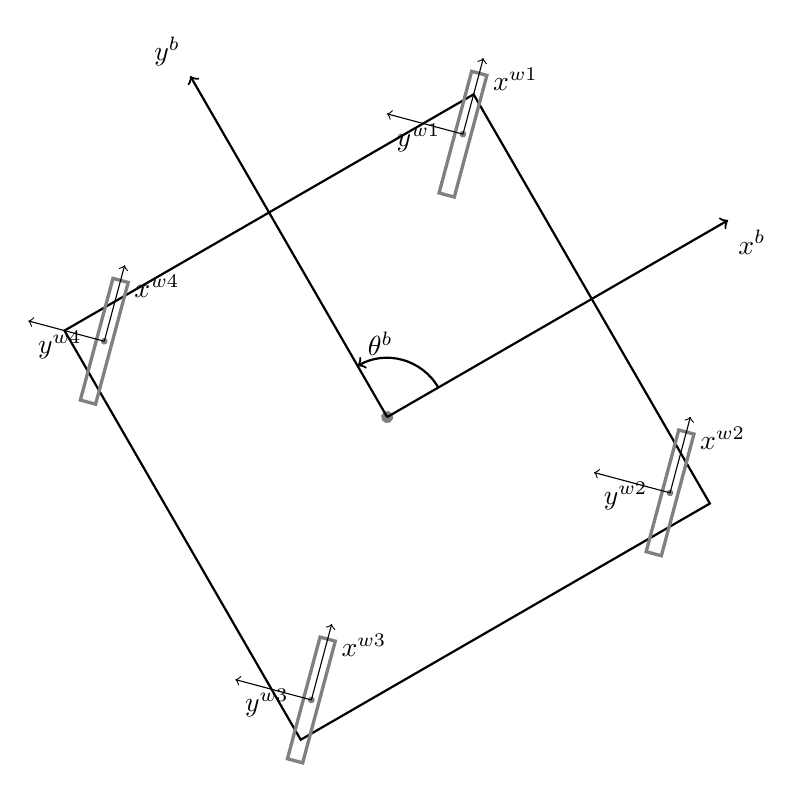
\begin{tikzpicture}[rotate=30 ]
			                \pic[rotate=30 ] at(0,0) {platform};
			                \pic[rotate=75 ] at(2.63,2.63) {wheelFrame={1}};
			                \pic[rotate=75 ] at(2.63,-2.63) {wheelFrame={2}};
			                \pic[rotate=75 ] at(-2.63,2.63) {wheelFrame={4}};
			                \pic[rotate=75 ] at(-2.63,-2.63) {wheelFrame={3}};
			                
		                \end{tikzpicture}
		            }
                    \caption{Task space velocity}
                    \label{fig:sub2}
                \end{subfigure}
            \end{figure}

\end{frame}


%%%%%%%%%%%%%%%%%%%%%%%%%%%%%%%%%%%%%%%%%%%%%%%%%%%%%%%%%%%%%%%%%
\begin{frame}{Kinematics Constraints}
    Basically there is only one kinematic constraint:\\\textbf{The wheel drives without slipping or lateral skidding}\\
    Which means the wheel contact point with ground has 0 tangential and normal velocity. $v_{ti}=0, v_{ni}=0$
    \begin{figure}
        \centering
        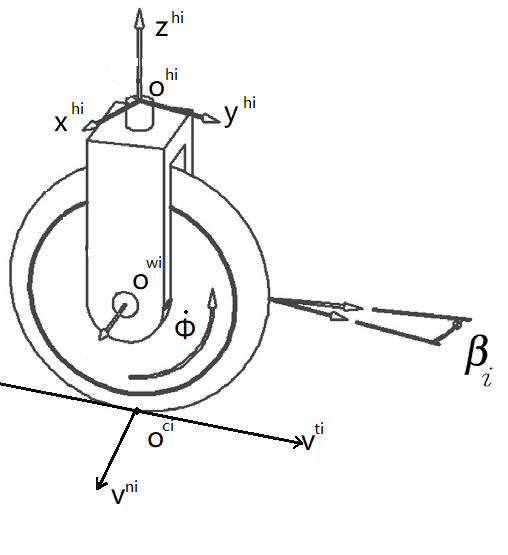
\includegraphics[width=0.5\textwidth]{Figure/wheel.png}
        \label{fig:wheel}
    \end{figure}
\end{frame}
%%%%%%%%%%%%%%%%%%%%%%%%%%%%%%%%%%%%%%%%%%%%%%%%%%%%%%%%%%%%%%%%%



%%%%%%%%%%%%%%%%%%%%%%%%%%%%%%%%%%%%%%%%%%%%%%%%%%%%%%%%%%%%%%%%%
\begin{frame}{Kinematics Constraints}
    From the $v_{ti}=0, v_{ni}=0$ constraint we can derive equations: 
    \begin{equation}\label{eq:2}
	\begin{split}
	\beta_i &= tan^{-1}(\frac{\dot{y^b}+h_{xi}\dot{\theta^b}}{\dot{x^b}-h_{yi}\dot{\theta^b}})
	\end{split}
\end{equation}

\begin{equation}\label{eq:3}
	\begin{split}
	\dot{\beta_i} &= \frac{-g(\dot{\beta_i})\ddot{\xi}}{\frac{dg(\dot{\beta_i})}{d\beta_i}\dot{\xi}}=\frac{\partial\beta_i}{\partial\dot{x}^b}\ddot{x}^b+\frac{\partial\beta_i}{\partial\dot{y}^b}\ddot{y}^b +\frac{\partial\beta_i}{\partial\dot{\theta^b}}\ddot{\theta}^b
	=f_{1i}(\dot{\xi^b})\ddot{\xi^b}
	\end{split}
\end{equation}

\begin{equation}\label{eq:4}
	\begin{split}
	\dot{\phi_i} &= \frac{1}{r_w}[cos(\beta_i), sin(\beta_i), -h_{yi}cos(\beta_i)+h_{xi}sin(\beta_i)]\dot{\xi^b}=f_{2i}(\beta)\dot{\xi^b}
	\end{split}
\end{equation}

These equations combined are called inverse kinematics(IK). Given task space command $\dot{\xi}=[\dot{x},\dot{y},\dot{\theta}]$ and $\ddot{\xi}=[\ddot{x},\ddot{y},\ddot{\theta}]$. We can use the IK to get the corresponding steering angle $\beta$, steering velocity $\dot{\beta}$ and driving speed $\dot{\phi}$
\end{frame}
%%%%%%%%%%%%%%%%%%%%%%%%%%%%%%%%%%%%%%%%%%%%%%%%%%%%%%%%%%%%%%%%%
\begin{frame}{Instantaneous center of rotation (ICR)}
    Another interpretation for the kinematics is that, if the \textbf{no slipping or lateral skidding} constraint is met. Then at each instant the motion of the robot can be viewed as an instantaneous rotation around the ICR
    \begin{figure}
	\begin{center}
	\resizebox{4cm}{!}
    {
		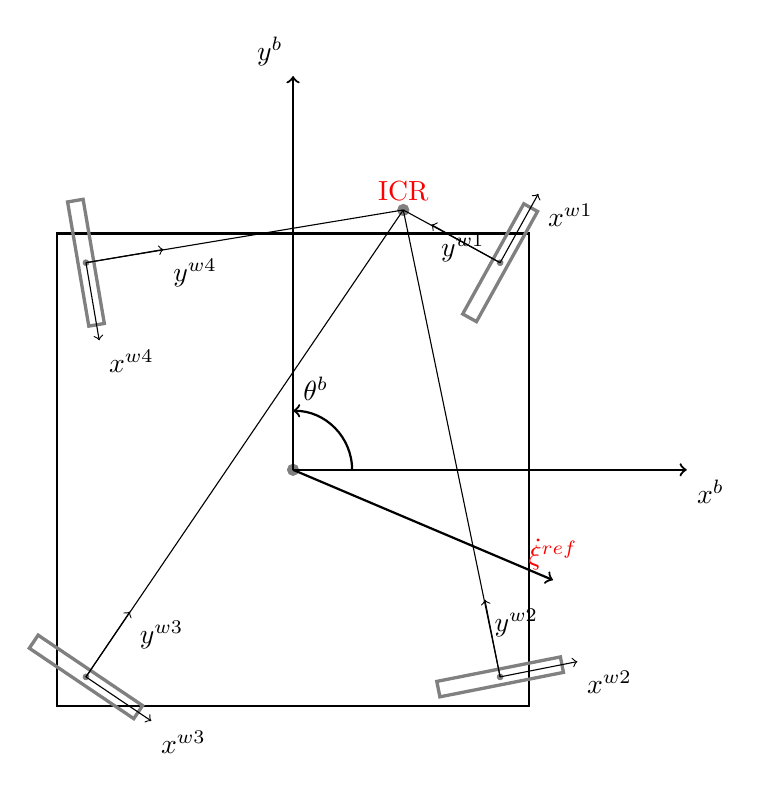
\begin{tikzpicture}
			\pic at(0,0) {platform};
			\pic[rotate=61] at(2.63,2.63) {wheelFrame={1}};
			\pic[rotate=11.2] at(2.63,-2.63) {wheelFrame={2}};
			\pic[rotate=-80.3] at(-2.63,2.63) {wheelFrame={4}};
			\pic[rotate=-34] at(-2.63,-2.63) {wheelFrame={3}};		
			\filldraw [gray] (1.4,3.3) circle (2pt) node[above,text=red]{ICR};
			\draw [rotate=-90, thick, ->] (0,0) -- (1.4,3.3) node[above,text=red]{$\dot{\xi}^{ref}$};
			\draw (2.63,2.63) -- (1.4,3.3);
			\draw (2.63,-2.63) -- (1.4,3.3);
			\draw (-2.63,-2.63) -- (1.4,3.3);
			\draw (-2.63,2.63) -- (1.4,3.3);
		\end{tikzpicture}
		}
	\end{center}
	\caption{Instantaneous Center of Rotation}
\end{figure}
Conclusion: At each time instant, the y axles of all the wheels are concurrent at the ICR.
\end{frame}

%%%%%%%%%%%%%%%%%%%%%%%%%%%%%%%%%%%%%%%%%%%%%%%%%%%%%%%%%%%%%%%%%
\section{Problem Identification}
%%%%%%%%%%%%%%%%%%%%%%%%%%%%%%%%%%%%%%%%%%%%%%%%%%%%%%%%%%%%%%%%%

\begin{frame}{Inconsistency}
    In cases like obstacle avoidance, inconsistent task space command could happen. Huge acceleration on steering is required to conduct this sudden change in 1 control cycle (0.002s).
    The wheel motor will be broken/locked\\
    e.g. Pedestrian avoiding\\
    \begin{equation}
        \dot{\xi}^n=[1,0,0] - > \dot{\xi}^{n+1}=[0,1,0]
    \end{equation}
    
   
\end{frame}
%%%%%%%%%%%%%%%%%%%%%%%%%%%%%%%%%%%%%%%%%%%%%%%%%%%%%%%%%%%%%%%%%
\begin{frame}{Inconsistency}
 \begin{figure}
	\begin{center}
	\resizebox{5cm}{!}
    {
		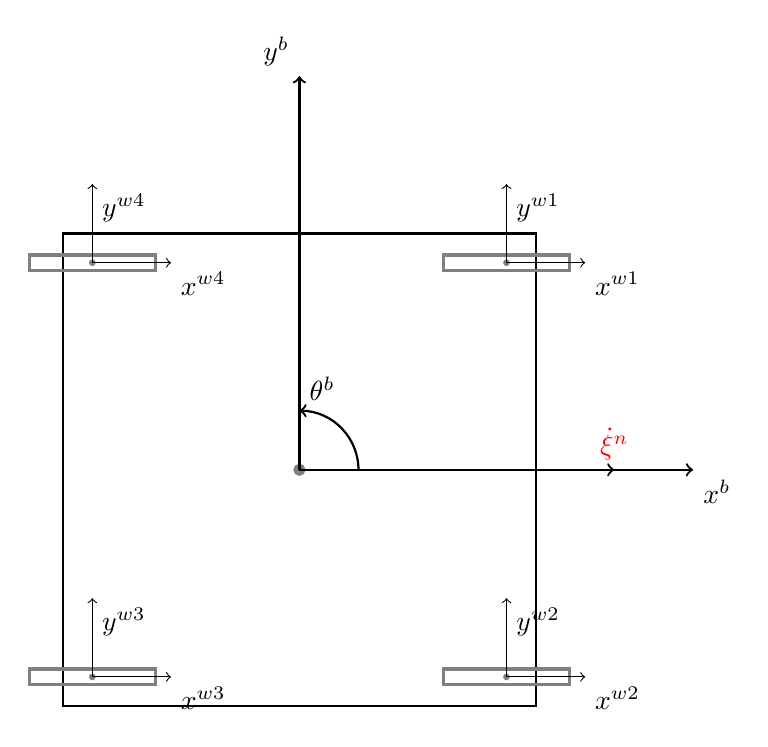
\begin{tikzpicture}
			\pic at(0,0) {platform};
			\pic[rotate=0] at(2.63,2.63) {wheelFrame={1}};
			\pic[rotate=0] at(2.63,-2.63) {wheelFrame={2}};
			\pic[rotate=0] at(-2.63,2.63) {wheelFrame={4}};
			\pic[rotate=0] at(-2.63,-2.63) {wheelFrame={3}};		
			%\filldraw [gray] (1.4,3.3) circle (2pt) node[above,text=red]{ICR};
			\draw [rotate=0, thick, ->] (0,0) -- (4,0) node[above,text=red]{$\dot{\xi}^{n}$};
% 			\draw (2.63,2.63) -- (1.4,3.3);
% 			\draw (2.63,-2.63) -- (1.4,3.3);
% 			\draw (-2.63,-2.63) -- (1.4,3.3);
% 			\draw (-2.63,2.63) -- (1.4,3.3);
		\end{tikzpicture}
		}
	\end{center}
	\caption{$\dot{\xi}^n=[1,0,0]$}
\end{figure}
\end{frame}
%%%%%%%%%%%%%%%%%%%%%%%%%%%%%%%%%%%%%%%%%%%%%%%%%%%%%%%%%%%%%%%%%
\begin{frame}{Inconsistency}
 \begin{figure}
	\begin{center}
	\resizebox{5cm}{!}
    {
		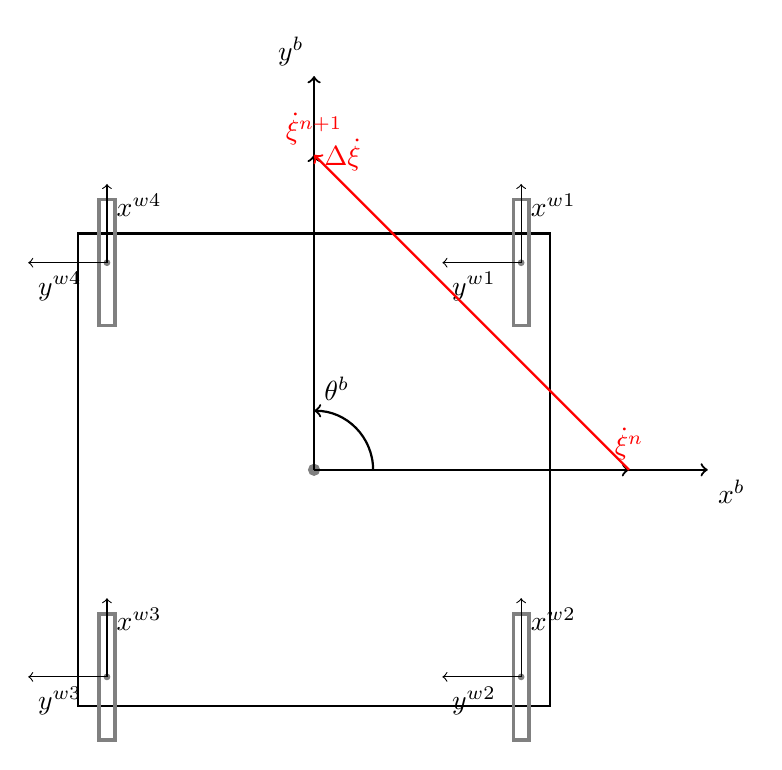
\begin{tikzpicture}
			\pic at(0,0) {platform};
			\pic[rotate=90] at(2.63,2.63) {wheelFrame={1}};
			\pic[rotate=90] at(2.63,-2.63) {wheelFrame={2}};
			\pic[rotate=90] at(-2.63,2.63) {wheelFrame={4}};
			\pic[rotate=90] at(-2.63,-2.63) {wheelFrame={3}};		
      %\filldraw [gray] (1.4,3.3) circle (2pt) node[above,text=red]{ICR};
      \draw [rotate=0, thick, ->] (0,0) -- (4,0) node[above,text=red]{$\dot{\xi}^{n}$};
      \draw [rotate=90, thick, ->] (0,0) -- (4,0) node[above,text=red]{$\dot{\xi}^{n+1}$};
      \draw [red,thick, ->] (4,0) -- (0,4) node[anchor=west,text=red]{$\Delta\dot{\xi}$};
% 			\draw (2.63,2.63) -- (1.4,3.3);
% 			\draw (2.63,-2.63) -- (1.4,3.3);
% 			\draw (-2.63,-2.63) -- (1.4,3.3);
% 			\draw (-2.63,2.63) -- (1.4,3.3);
		\end{tikzpicture}
		}
	\end{center}
	\caption{$\dot{\xi}^n=[0,1,0]$}
\end{figure}
\end{frame}

%%%%%%%%%%%%%%%%%%%%%%%%%%%%%%%%%%%%%%%%%%%%%%%%%%%%%%%%%%%%%%%%%
\begin{frame}{Inconsistency}
    We can also apply the ICR interpretation on the inconsistency problem. \\
    \textbf{Inconsistency task space command corresponding to a huge change of ICR position}\\
    e.g.:
    \begin{equation}
        \dot{\xi}^n=[3.3,-1.4,1] - > \dot{\xi}^{n+1}=[0,0,1]
    \end{equation}
\end{frame}

%%%%%%%%%%%%%%%%%%%%%%%%%%%%%%%%%%%%%%%%%%%%%%%%%%%%%%%%%%%%%%%%%
\begin{frame}{Inconsistency}
  \begin{figure}
	\begin{center}
	\resizebox{5cm}{!}
    {
		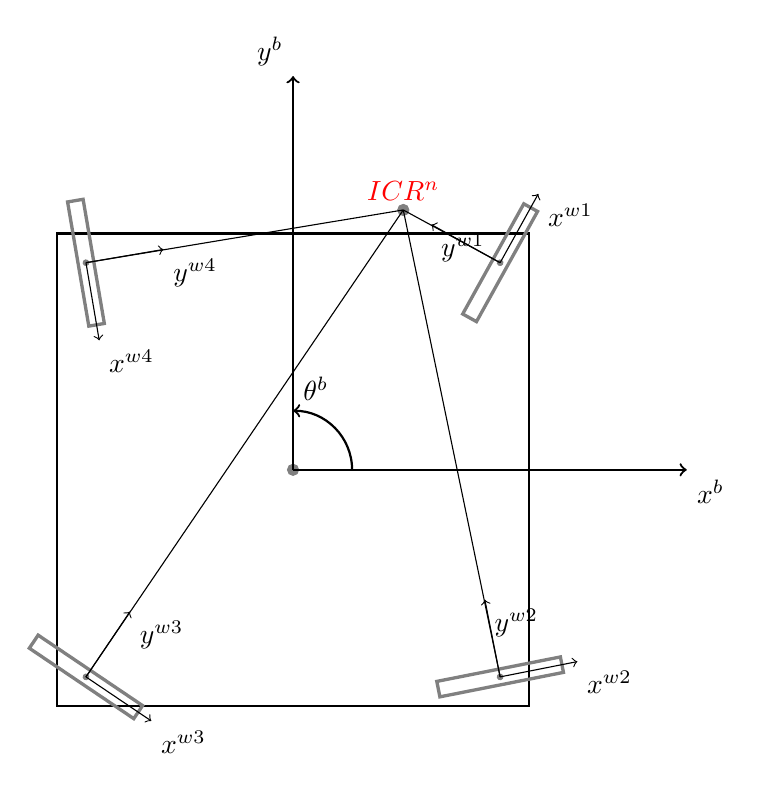
\begin{tikzpicture}
			\pic at(0,0) {platform};
			\pic[rotate=61] at(2.63,2.63) {wheelFrame={1}};
			\pic[rotate=11.2] at(2.63,-2.63) {wheelFrame={2}};
			\pic[rotate=-80.3] at(-2.63,2.63) {wheelFrame={4}};
			\pic[rotate=-34] at(-2.63,-2.63) {wheelFrame={3}};		
			\filldraw [gray] (1.4,3.3) circle (2pt) node[above,text=red]{$ICR^n$};
			%\draw [rotate=-90, thick, ->] (0,0) -- (1.4,3.3) node[above,text=red]{$\dot{\xi}^{ref}$};
			\draw (2.63,2.63) -- (1.4,3.3);
			\draw (2.63,-2.63) -- (1.4,3.3);
			\draw (-2.63,-2.63) -- (1.4,3.3);
			\draw (-2.63,2.63) -- (1.4,3.3);
		\end{tikzpicture}
		}
	\end{center}
	\caption{$\dot{\xi}^n=[3.3,-1.4,1]$}
\end{figure}
\end{frame}


%%%%%%%%%%%%%%%%%%%%%%%%%%%%%%%%%%%%%%%%%%%%%%%%%%%%%%%%%%%%%%%%%

\begin{frame}{Inconsistency}
     \begin{figure}
	\begin{center}
	\resizebox{5cm}{!}
    {
		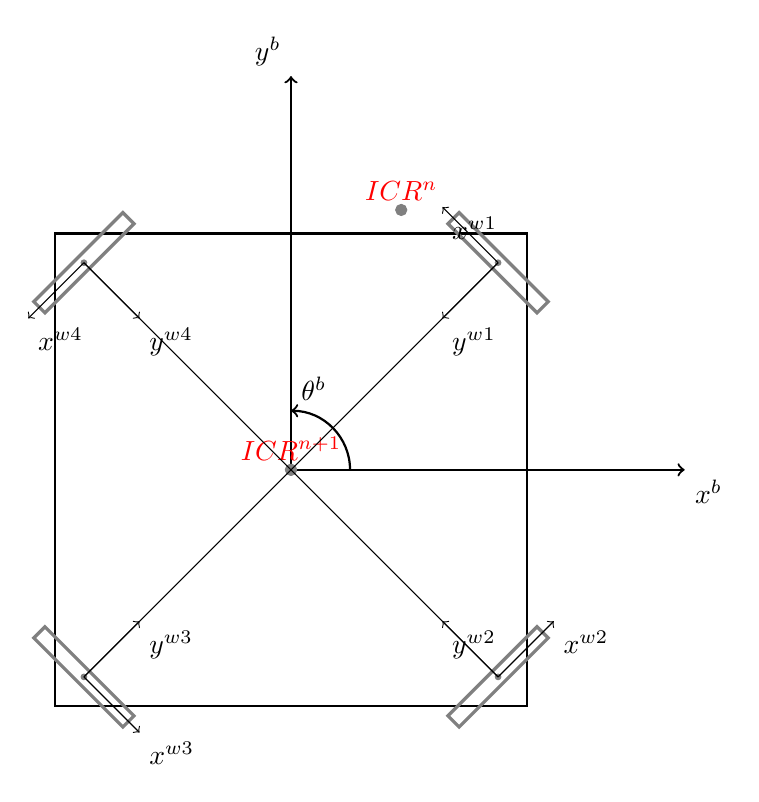
\begin{tikzpicture}
			\pic at(0,0) {platform};
			\pic[rotate=135] at(2.63,2.63) {wheelFrame={1}};
			\pic[rotate=45] at(2.63,-2.63) {wheelFrame={2}};
			\pic[rotate=-135] at(-2.63,2.63) {wheelFrame={4}};
      \pic[rotate=-45] at(-2.63,-2.63) {wheelFrame={3}};	
      \filldraw [gray] (1.4,3.3) circle (2pt) node[above,text=red]{$ICR^n$};	
			\filldraw [gray] (0,0) circle (2pt) node[above,text=red]{$ICR^{n+1}$};
			%\draw [rotate=-90, thick, ->] (0,0) -- (1.4,3.3) node[above,text=red]{$\dot{\xi}^{ref}$};
			\draw (2.63,2.63) -- (0,0);
			\draw (2.63,-2.63) -- (0,0);
			\draw (-2.63,-2.63) -- (0,0);
			\draw (-2.63,2.63) -- (0,0);
		\end{tikzpicture}
		}
	\end{center}
	\caption{$\dot{\xi}^{n+1}=[0,0,1]$}
\end{figure}
\end{frame}
%%%%%%%%%%%%%%%%%%%%%%%%%%%%%%%%%%%%%%%%%%%%%%%%%%%%%%%%%%%%%%%%%
\section{Solutions}
%%%%%%%%%%%%%%%%%%%%%%%%%%%%%%%%%%%%%%%%%%%%%%%%%%%%%%%%%%%%%%%%%
\begin{frame}{How to solve inconsistency?}
The inconsistemcy problem is due to the fact that kinematic model ignores the dynamic. 
\metroset{block=fill}

\begin{block}{Solution}
  Include dynamic constraints in the control logic.
\end{block}
 
\end{frame}

%%%%%%%%%%%%%%%%%%%%%%%%%%%%%%%%%%%%%%%%%%%%%%%%%%%%%%%%%%%%%%%%%
\begin{frame}{Approximation based Inverse Kinematic control}
  If we look back at the first instance, we can see that the difference $\Delta\dot{\xi}$ between current control cycle velocity and 
  next control cycle reference velocity is huge. Which means a big change of task space velocity corresponding to a big change 
  of joint configuration. 

  \begin{columns}[T,onlytextwidth]
    \column{0.4\textwidth}
    \metroset{block=fill}
    \begin{block}{Idea}
      Scaling down the amount of changing $\Delta\dot{\xi},\Delta\ddot{\xi}$ based on the dynamic cosntraint.
    \end{block}

      But what is the relationship between $\Delta\dot{\xi},\Delta\ddot{\xi}$ and joint acceleration and how much shall we scale down?

    \column{0.6\textwidth}

    \begin{figure}
      \begin{center}
      \resizebox{5cm}{!}
        {
        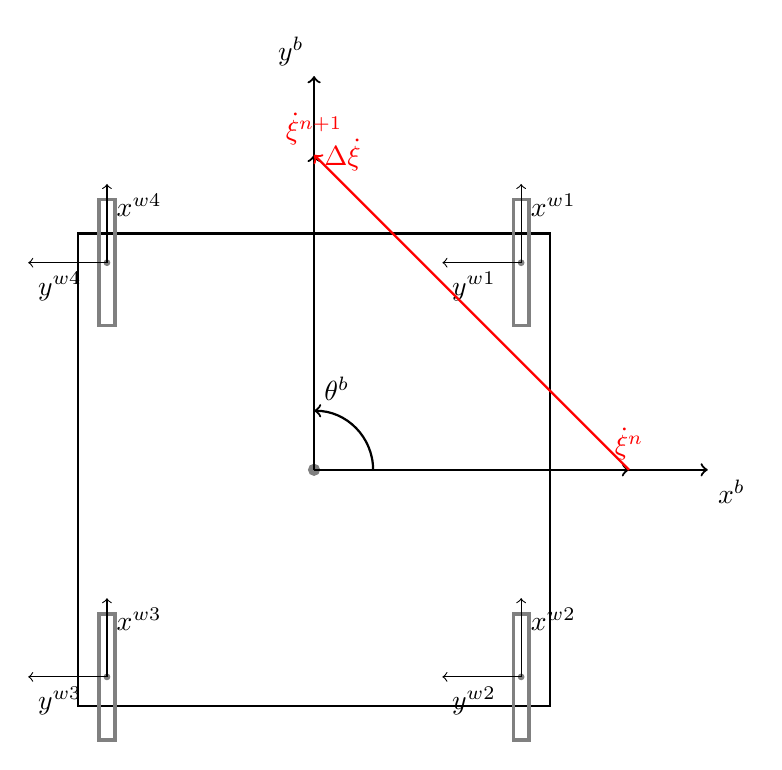
\begin{tikzpicture}
          \pic at(0,0) {platform};
          \pic[rotate=90] at(2.63,2.63) {wheelFrame={1}};
          \pic[rotate=90] at(2.63,-2.63) {wheelFrame={2}};
          \pic[rotate=90] at(-2.63,2.63) {wheelFrame={4}};
          \pic[rotate=90] at(-2.63,-2.63) {wheelFrame={3}};		
          %\filldraw [gray] (1.4,3.3) circle (2pt) node[above,text=red]{ICR};
          \draw [rotate=0, thick, ->] (0,0) -- (4,0) node[above,text=red]{$\dot{\xi}^{n}$};
          \draw [rotate=90, thick, ->] (0,0) -- (4,0) node[above,text=red]{$\dot{\xi}^{n+1}$};
          \draw [red,thick, ->] (4,0) -- (0,4) node[anchor=west,text=red]{$\Delta\dot{\xi}$};
    % 			\draw (2.63,2.63) -- (1.4,3.3);
    % 			\draw (2.63,-2.63) -- (1.4,3.3);
    % 			\draw (-2.63,-2.63) -- (1.4,3.3);
    % 			\draw (-2.63,2.63) -- (1.4,3.3);
        \end{tikzpicture}
        }
      \end{center}
      \caption{$\Delta\dot{\xi}$}
    \end{figure}

  \end{columns}

  
  
\end{frame}

%%%%%%%%%%%%%%%%%%%%%%%%%%%%%%%%%%%%%%%%%%%%%%%%%%%%%%%%%%%%%%%%%
\begin{frame}{Approximation based Inverse Kinematic control}
Linearize the kinematics about the current state of the mobile platform. Then we have a linear relationship between 
$\Delta\dot{\xi},\Delta\ddot{\xi}$ and joint acceleration

\begin{equation}\label{eq:deltaRelation}
  \begin{split}
      \ddot{\beta}^{n+1}&=\Delta\dot{\beta}_i/\Delta T=\frac{1}{\Delta T}f_{1i}(\dot{\xi}^n)\Delta\ddot{\xi}\\
      \ddot{\phi}^{n+1}&=\Delta\dot{\phi}_i/\Delta T=\frac{1}{\Delta T}f_{2i}(\beta^n)\Delta\dot{\xi}
  \end{split}
\end{equation}

Base on the above equition, we can detect violation of acceleration limits, and scale down the corresponding term 
$\Delta\dot{\xi}_{new}= \frac{\ddot{\phi}_{max}}{\ddot{\phi}}\Delta\dot{\xi}$.\\
And then calculate the new command $\dot{\xi}^{n+1}_{new}=\dot{\xi}^n+\Delta\dot{\xi}_{new}$
\end{frame}
%%%%%%%%%%%%%%%%%%%%%%%%%%%%%%%%%%%%%%%%%%%%%%%%%%%%%%%%%%%%%%%%%
\begin{frame}{Approximation based Inverse Kinematic control}
  \begin{figure}
    \begin{center}
    \resizebox{7cm}{!}
      {
      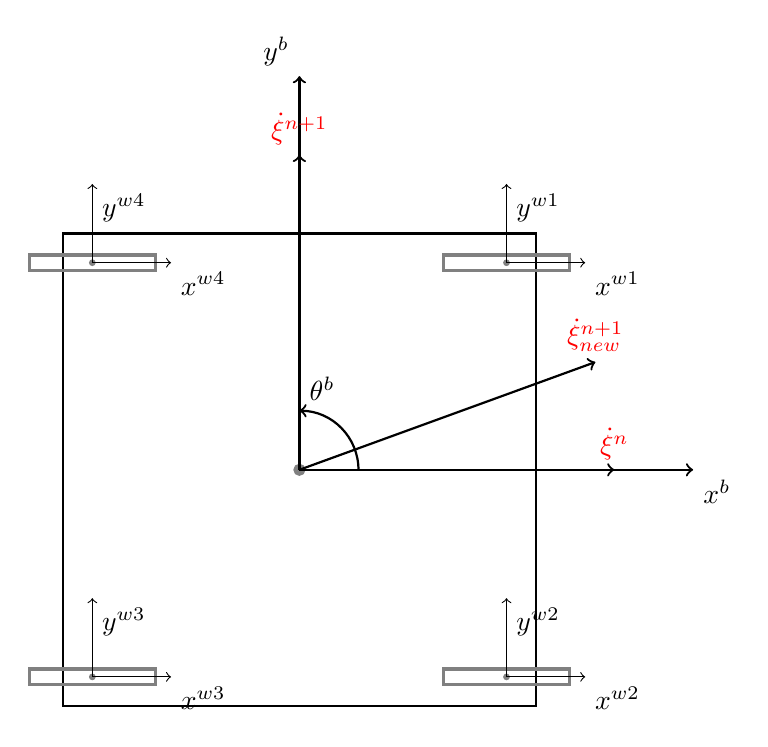
\begin{tikzpicture}
        \pic at(0,0) {platform};
        \pic[rotate=0] at(2.63,2.63) {wheelFrame={1}};
        \pic[rotate=0] at(2.63,-2.63) {wheelFrame={2}};
        \pic[rotate=0] at(-2.63,2.63) {wheelFrame={4}};
        \pic[rotate=0] at(-2.63,-2.63) {wheelFrame={3}};		
        %\filldraw [gray] (1.4,3.3) circle (2pt) node[above,text=red]{ICR};
        \draw [rotate=0, thick, ->] (0,0) -- (4,0) node[above,text=red]{$\dot{\xi}^{n}$};
        \draw [rotate=20, thick, ->] (0,0) -- (4,0) node[above,text=red]{$\dot{\xi}^{n+1}_{new}$};
        \draw [rotate=90, thick, ->] (0,0) -- (4,0) node[above,text=red]{$\dot{\xi}^{n+1}$};
        % \draw [red,thick, ->] (4,0) -- (0,4) node[anchor=west,text=red]{$\Delta\dot{\xi}$};
  % 			\draw (2.63,2.63) -- (1.4,3.3);
  % 			\draw (2.63,-2.63) -- (1.4,3.3);
  % 			\draw (-2.63,-2.63) -- (1.4,3.3);
  % 			\draw (-2.63,2.63) -- (1.4,3.3);
      \end{tikzpicture}
      }
    \end{center}
    \caption{Scaling process}
  \end{figure}
\end{frame}


%%%%%%%%%%%%%%%%%%%%%%%%%%%%%%%%%%%%%%%%%%%%%%%%%%%%%%%%%%%%%%%%%

\begin{frame}{Approximation based Inverse Kinematic control}
  \begin{figure}
    \begin{center}
    \resizebox{7cm}{!}
      {
      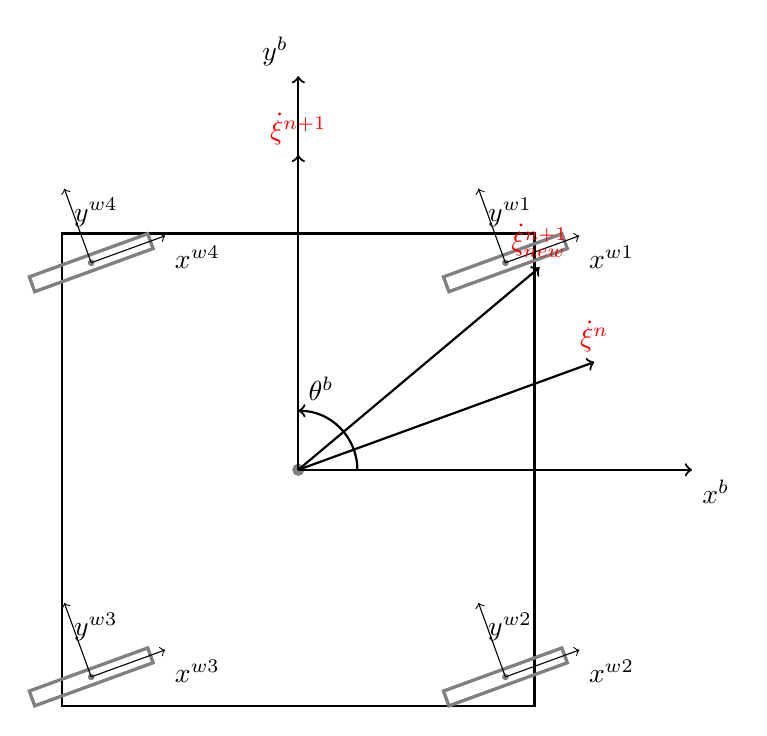
\begin{tikzpicture}
        \pic at(0,0) {platform};
        \pic[rotate=20] at(2.63,2.63) {wheelFrame={1}};
        \pic[rotate=20] at(2.63,-2.63) {wheelFrame={2}};
        \pic[rotate=20] at(-2.63,2.63) {wheelFrame={4}};
        \pic[rotate=20] at(-2.63,-2.63) {wheelFrame={3}};		
        %\filldraw [gray] (1.4,3.3) circle (2pt) node[above,text=red]{ICR};
        \draw [rotate=20, thick, ->] (0,0) -- (4,0) node[above,text=red]{$\dot{\xi}^{n}$};
        \draw [rotate=40, thick, ->] (0,0) -- (4,0) node[above,text=red]{$\dot{\xi}^{n+1}_{new}$};
        \draw [rotate=90, thick, ->] (0,0) -- (4,0) node[above,text=red]{$\dot{\xi}^{n+1}$};
        % \draw [red,thick, ->] (4,0) -- (0,4) node[anchor=west,text=red]{$\Delta\dot{\xi}$};
  % 			\draw (2.63,2.63) -- (1.4,3.3);
  % 			\draw (2.63,-2.63) -- (1.4,3.3);
  % 			\draw (-2.63,-2.63) -- (1.4,3.3);
  % 			\draw (-2.63,2.63) -- (1.4,3.3);
      \end{tikzpicture}
      }
    \end{center}
    \caption{Scaling process}
  \end{figure}
\end{frame}


%%%%%%%%%%%%%%%%%%%%%%%%%%%%%%%%%%%%%%%%%%%%%%%%%%%%%%%%%%%%%%%%%

\begin{frame}{Approximation based Inverse Kinematic control}
  \begin{figure}
    \begin{center}
    \resizebox{7cm}{!}
      {
      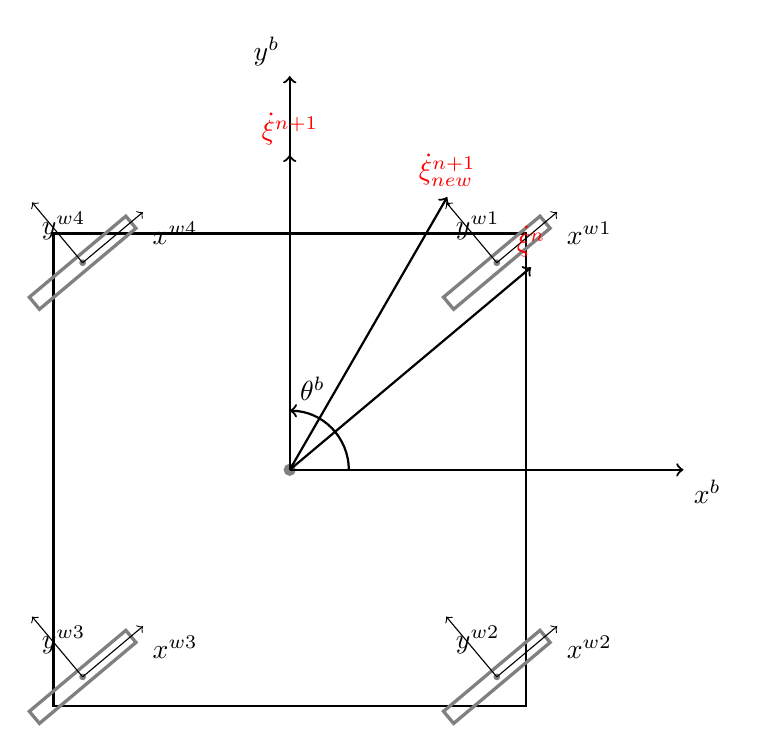
\begin{tikzpicture}
        \pic at(0,0) {platform};
        \pic[rotate=40] at(2.63,2.63) {wheelFrame={1}};
        \pic[rotate=40] at(2.63,-2.63) {wheelFrame={2}};
        \pic[rotate=40] at(-2.63,2.63) {wheelFrame={4}};
        \pic[rotate=40] at(-2.63,-2.63) {wheelFrame={3}};		
        %\filldraw [gray] (1.4,3.3) circle (2pt) node[above,text=red]{ICR};
        \draw [rotate=40, thick, ->] (0,0) -- (4,0) node[above,text=red]{$\dot{\xi}^{n}$};
        \draw [rotate=60, thick, ->] (0,0) -- (4,0) node[above,text=red]{$\dot{\xi}^{n+1}_{new}$};
        \draw [rotate=90, thick, ->] (0,0) -- (4,0) node[above,text=red]{$\dot{\xi}^{n+1}$};
        % \draw [red,thick, ->] (4,0) -- (0,4) node[anchor=west,text=red]{$\Delta\dot{\xi}$};
  % 			\draw (2.63,2.63) -- (1.4,3.3);
  % 			\draw (2.63,-2.63) -- (1.4,3.3);
  % 			\draw (-2.63,-2.63) -- (1.4,3.3);
  % 			\draw (-2.63,2.63) -- (1.4,3.3);
      \end{tikzpicture}
      }
    \end{center}
    \caption{Scaling process}
  \end{figure}
\end{frame}

%%%%%%%%%%%%%%%%%%%%%%%%%%%%%%%%%%%%%%%%%%%%%%%%%%%%%%%%%%%%%%%%%

\begin{frame}{Approximation based Inverse Kinematic control}
  \begin{figure}
    \begin{center}
    \resizebox{7cm}{!}
      {
      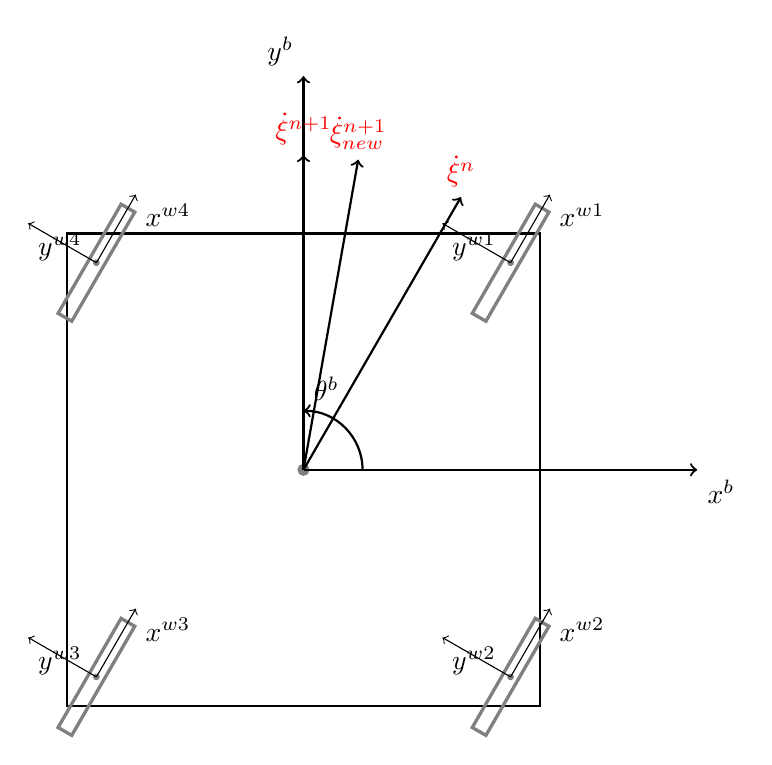
\begin{tikzpicture}
        \pic at(0,0) {platform};
        \pic[rotate=60] at(2.63,2.63) {wheelFrame={1}};
        \pic[rotate=60] at(2.63,-2.63) {wheelFrame={2}};
        \pic[rotate=60] at(-2.63,2.63) {wheelFrame={4}};
        \pic[rotate=60] at(-2.63,-2.63) {wheelFrame={3}};		
        %\filldraw [gray] (1.4,3.3) circle (2pt) node[above,text=red]{ICR};
        \draw [rotate=60, thick, ->] (0,0) -- (4,0) node[above,text=red]{$\dot{\xi}^{n}$};
        \draw [rotate=80, thick, ->] (0,0) -- (4,0) node[above,text=red]{$\dot{\xi}^{n+1}_{new}$};
        \draw [rotate=90, thick, ->] (0,0) -- (4,0) node[above,text=red]{$\dot{\xi}^{n+1}$};
        % \draw [red,thick, ->] (4,0) -- (0,4) node[anchor=west,text=red]{$\Delta\dot{\xi}$};
  % 			\draw (2.63,2.63) -- (1.4,3.3);
  % 			\draw (2.63,-2.63) -- (1.4,3.3);
  % 			\draw (-2.63,-2.63) -- (1.4,3.3);
  % 			\draw (-2.63,2.63) -- (1.4,3.3);
      \end{tikzpicture}
      }
    \end{center}
    \caption{Scaling process}
  \end{figure}
\end{frame}


%%%%%%%%%%%%%%%%%%%%%%%%%%%%%%%%%%%%%%%%%%%%%%%%%%%%%%%%%%%%%%%%%
\begin{frame}{Approximation based Inverse Kinematic control}
\metroset{block=fill}
The linearized approximation is relative accurate in most cases. But the kinematics have sigularity configurations, when 
the task space velocity command getting close to these configurations, approximation error increase significantly.
\begin{columns}
  \column{0.4\textwidth}
  \begin{block}{Limitation}
  Expressed in ICR form, the approximation error increase when ICR getting close to the platform
  \end{block}
  \textbf{Need another method as complementary}
  \column{0.5\textwidth}
    \begin{figure}
        \centering
        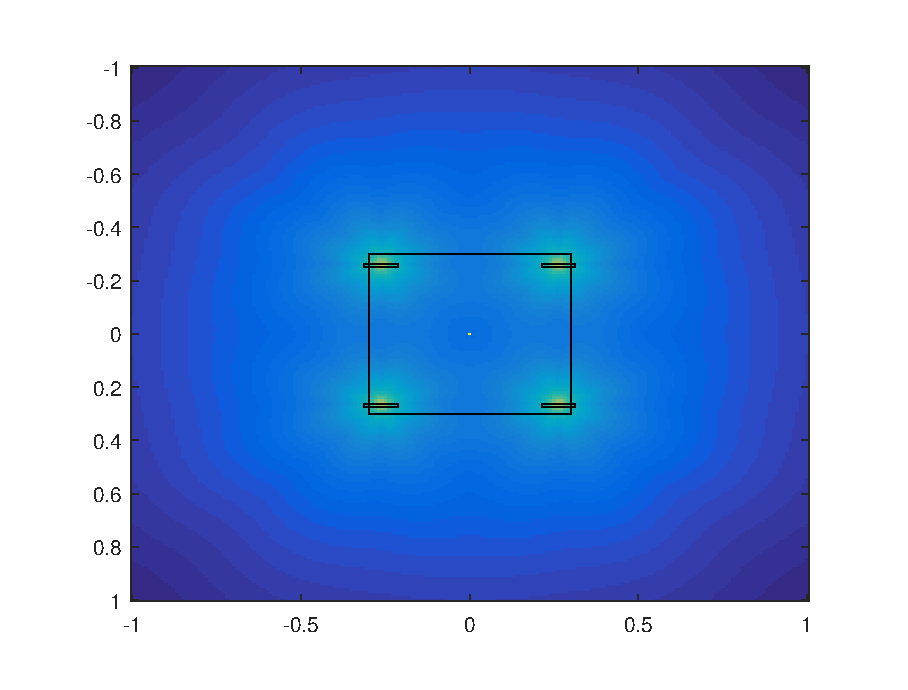
\includegraphics[width=\textwidth]{Figure/approximationError.eps}
        \caption{Approximation error}
        \label{fig:appError}
    \end{figure}
\end{columns}

\end{frame}
%%%%%%%%%%%%%%%%%%%%%%%%%%%%%%%%%%%%%%%%%%%%%%%%%%%%%%%%%%%%%%%%%
%%%%%%%%%%%%%%%%%%%%%%%%%%%%%%%%%%%%%%%%%%%%%%%%%%%%%%%%%%%%%%%%%
%%%%%%%%%%%%%%%%%%%%%%%%%%%%%%%%%%%%%%%%%%%%%%%%%%%%%%%%%%%%%%%%%
%%%%%%%%%%%%%%%%%%%%%%%%%%%%%%%%%%%%%%%%%%%%%%%%%%%%%%%%%%%%%%%%%

\begin{frame}{ICR optimization control}
    As mentioned before, the effect of inconsistency in ICR space is a big jump of reference ICR. Then our mission is to find a optimal $ICR^{n+1}_{new}$ so that is respect the joint acceleration limit and as close to the reference ICR as possible.
    \begin{columns}
      \column{0.4\textwidth}
      \metroset{block=fill}
        \begin{block}{Idea}
            Form an optimization problem with the distance between $ICR^n$ and $ICR^{n+1}_{new}$ as cost function. and the acceleration limit projected on the ICR space as linear inequality constraints.
        \end{block}
        \column{0.5\textwidth}
        \begin{figure}
	\centering
	\resizebox{6cm}{!}
      {
	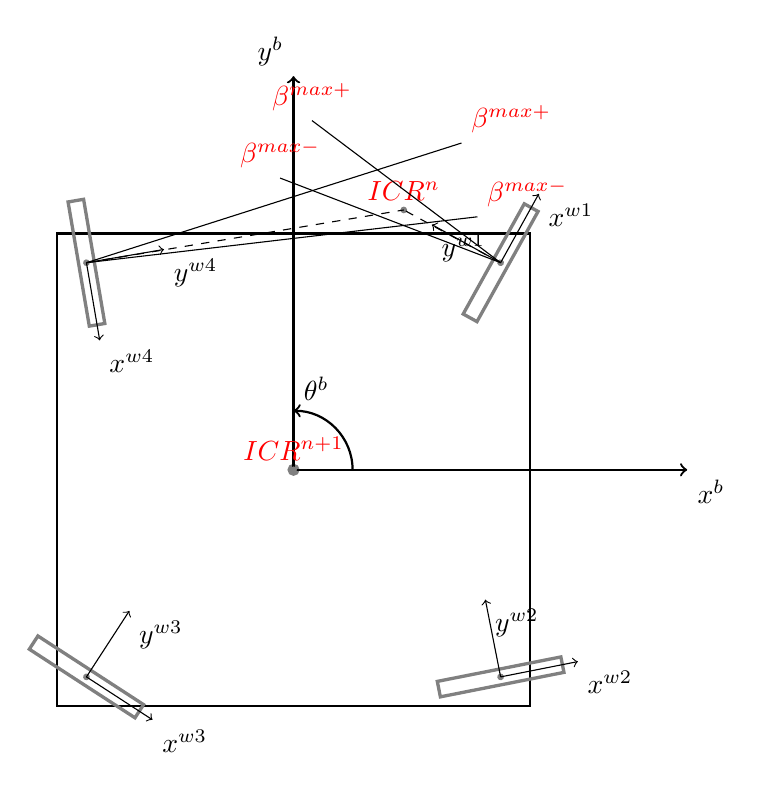
\begin{tikzpicture}
			\pic at(0,0) {platform};
			\pic[rotate=61] at(2.63,2.63) {wheelFrame={1}};
			\pic[rotate=11.2] at(2.63,-2.63) {wheelFrame={2}};
			\pic[rotate=-80.3] at(-2.63,2.63) {wheelFrame={4}};
			\pic[rotate=-33] at(-2.63,-2.63) {wheelFrame={3}};		
			\filldraw [gray] (1.4,3.3) circle (1pt) node[above,text=red]{$ICR^n$};
			\filldraw [gray] (0,0) circle (1pt) node[above,text=red]{$ICR^{n+1}$};
			%\draw [rotate=-90, thick, ->] (0,0) -- (1.4,3.3) node[above,text=red]{$\dot{\xi}^{ref}$};
			\draw[dashed] (2.63,2.63)  -- (1.4,3.3);
			\draw (2.63,2.63)  -- +(143:3) node[above,text=red]{$\beta^{max+}$};
			\draw (2.63,2.63)  -- +(159:3) node[above,text=red]{$\beta^{max-}$};
			%\draw (2.63,-2.63)  -- +(101.2:8);
			%\draw (-2.63,-2.63) -- +(57:9);
			\draw[dashed] (-2.63,2.63)  -- (1.4,3.3);
			\draw (-2.63,2.63)  -- +(17.7:5)node[anchor=south west,text=red]{$\beta^{max+}$};
			\draw (-2.63,2.63)  -- +(6.7:5)node[anchor=south west,text=red]{$\beta^{max-}$};
	\end{tikzpicture}
	}
	\caption{}
	\label{}
\end{figure}

    \end{columns}
    
\end{frame}

%%%%%%%%%%%%%%%%%%%%%%%%%%%%%%%%%%%%%%%%%%%%%%%%%%%%%%%%%%%%%%%%%
\begin{frame}{ICR optimization method}
    A QP problem with 8 linear inequality constraints.
      \begin{equation} \label{eq:QP}
	    \begin{split}
		\underset{ICR_{next}}{\textbf{minimize}} \qquad &\parallel ICR_{next}-ICR_{curr}\parallel_2^2\\
		\underset{i=1:4}{\textbf{subject} \quad \textbf{to}} \qquad &(-1)^{q_i(min)}A_{i(min)}(ICR_{next}-hi)>=0\\
												  &(-1)^{q_i(max)+1}A_{i(max)}(ICR_{next}-hi)<=0
	    \end{split}
      \end{equation}
      Solve with an open source library of Active set method (QuadProg++)
      
    
\end{frame}
%%%%%%%%%%%%%%%%%%%%%%%%%%%%%%%%%%%%%%%%%%%%%%%%%%%%%%%%%%%%%%%%%
\begin{frame}{ICR optimization method}
    \begin{figure}
	\centering
	\resizebox{6cm}{!}
      {
	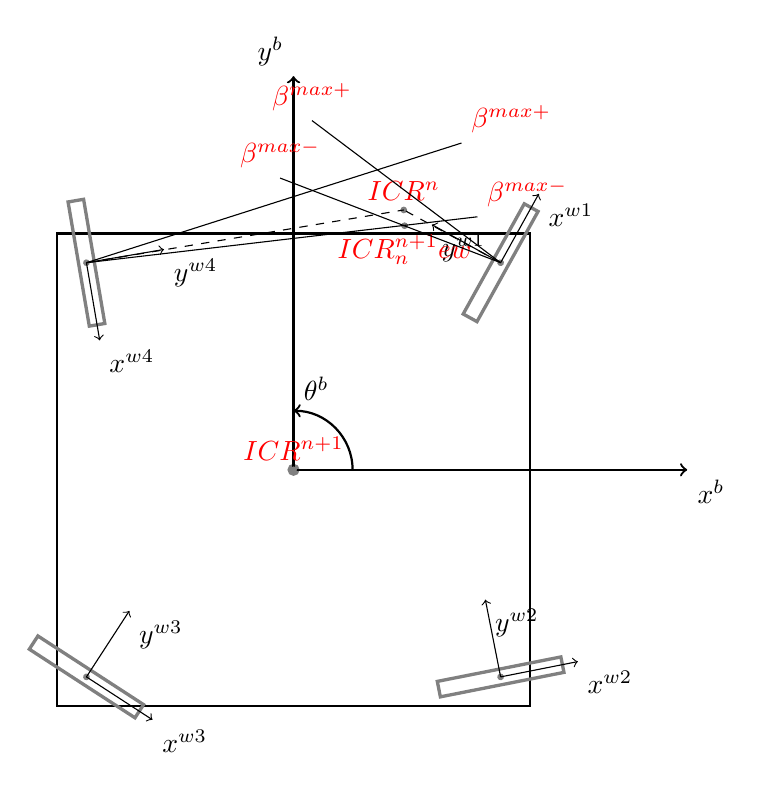
\begin{tikzpicture}
			\pic at(0,0) {platform};
			\pic[rotate=61] at(2.63,2.63) {wheelFrame={1}};
			\pic[rotate=11.2] at(2.63,-2.63) {wheelFrame={2}};
			\pic[rotate=-80.3] at(-2.63,2.63) {wheelFrame={4}};
			\pic[rotate=-33] at(-2.63,-2.63) {wheelFrame={3}};		
			\filldraw [gray] (1.4,3.3) circle (1pt) node[above,text=red]{$ICR^n$};
			\filldraw [gray] (0,0) circle (1pt) node[above,text=red]{$ICR^{n+1}$};
			\filldraw [gray] (1.41,3.1) circle (1pt) node[below,text=red]{$ICR^{n+1}_new$};
			%\draw [rotate=-90, thick, ->] (0,0) -- (1.4,3.3) node[above,text=red]{$\dot{\xi}^{ref}$};
			\draw[dashed] (2.63,2.63)  -- (1.4,3.3);
			\draw (2.63,2.63)  -- +(143:3) node[above,text=red]{$\beta^{max+}$};
			\draw (2.63,2.63)  -- +(159:3) node[above,text=red]{$\beta^{max-}$};
			%\draw (2.63,-2.63)  -- +(101.2:8);
			%\draw (-2.63,-2.63) -- +(57:9);
			\draw[dashed] (-2.63,2.63)  -- (1.4,3.3);
			\draw (-2.63,2.63)  -- +(17.7:5)node[anchor=south west,text=red]{$\beta^{max+}$};
			\draw (-2.63,2.63)  -- +(6.7:5)node[anchor=south west,text=red]{$\beta^{max-}$};
	\end{tikzpicture}
	}
	\caption{try to execute $\dot{\xi}=[0,0,1]$}
	\label{}
\end{figure}
\end{frame}

%%%%%%%%%%%%%%%%%%%%%%%%%%%%%%%%%%%%%%%%%%%%%%%%%%%%%%%%%%%%%%%%%
\begin{frame}{ICR optimization method}
     \begin{figure}
	\centering
	\resizebox{6cm}{!}
      {
	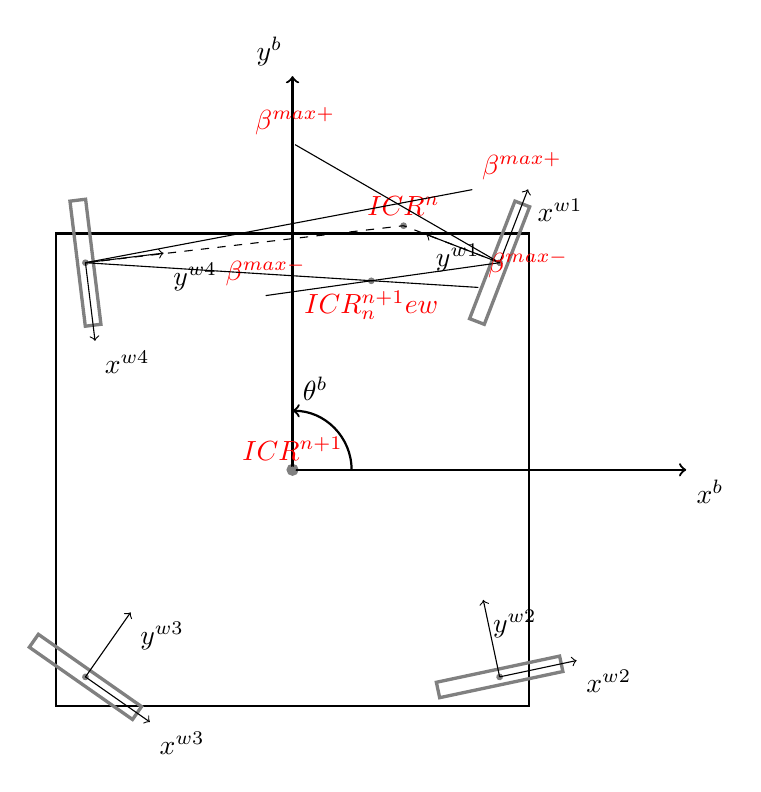
\begin{tikzpicture}
			\pic at(0,0) {platform};
			\pic[rotate=68.9] at(2.63,2.63) {wheelFrame={1}};
			\pic[rotate=12] at(2.63,-2.63) {wheelFrame={2}};
			\pic[rotate=-83] at(-2.63,2.63) {wheelFrame={4}};
			\pic[rotate=-35] at(-2.63,-2.63) {wheelFrame={3}};		
			\filldraw [gray] (1.41,3.1) circle (1pt) node[above,text=red]{$ICR^n$};
			\filldraw [gray] (0,0) circle (1pt) node[above,text=red]{$ICR^{n+1}$};
			\filldraw [gray] (1,2.4) circle (1pt) node[below,text=red]{$ICR^{n+1}_new$};
			%\draw [rotate=-90, thick, ->] (0,0) -- (1.4,3.3) node[above,text=red]{$\dot{\xi}^{ref}$};
			\draw[dashed] (2.63,2.63)  -- (1.41,3.1);
			\draw (2.63,2.63)  -- +(150:3) node[above,text=red]{$\beta^{max+}$};
			\draw (2.63,2.63)  -- +(188:3) node[above,text=red]{$\beta^{max-}$};
			%\draw (2.63,-2.63)  -- +(101.2:8);
			%\draw (-2.63,-2.63) -- +(57:9);
			\draw[dashed] (-2.63,2.63)  -- (1.41,3.1);
			\draw (-2.63,2.63)  -- +(10.7:5)node[anchor=south west,text=red]{$\beta^{max+}$};
			\draw (-2.63,2.63)  -- +(-3.6:5)node[anchor=south west,text=red]{$\beta^{max-}$};
	\end{tikzpicture}
	}
	\caption{try to execute $\dot{\xi}=[0,0,1]$}
	\label{}
\end{figure}
\end{frame}

%%%%%%%%%%%%%%%%%%%%%%%%%%%%%%%%%%%%%%%%%%%%%%%%%%%%%%%%%%%%%%%%%

\begin{frame}{ICR optimization method}
     \begin{figure}
	\centering
	\resizebox{6cm}{!}
      {
	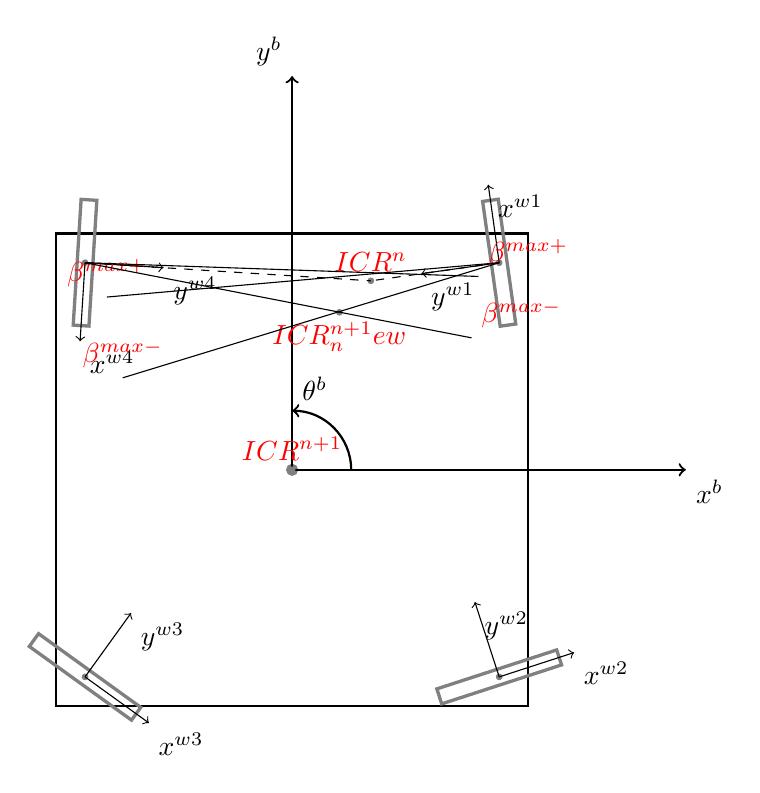
\begin{tikzpicture}
			\pic at(0,0) {platform};
			\pic[rotate=98] at(2.63,2.63) {wheelFrame={1}};
			\pic[rotate=18] at(2.63,-2.63) {wheelFrame={2}};
			\pic[rotate=-93.6] at(-2.63,2.63) {wheelFrame={4}};
			\pic[rotate=-35.8] at(-2.63,-2.63) {wheelFrame={3}};		
			\filldraw [gray] (1,2.4) circle (1pt) node[above,text=red]{$ICR^n$};
			\filldraw [gray] (0,0) circle (1pt) node[above,text=red]{$ICR^{n+1}$};
			\filldraw [gray] (0.6,2) circle (1pt) node[below,text=red]{$ICR^{n+1}_new$};
			%\draw [rotate=-90, thick, ->] (0,0) -- (1.4,3.3) node[above,text=red]{$\dot{\xi}^{ref}$};
			\draw[dashed] (2.63,2.63)  -- (1,2.4);
			\draw (2.63,2.63)  -- +(185:5) node[above,text=red]{$\beta^{max+}$};
			\draw (2.63,2.63)  -- +(197:5) node[above,text=red]{$\beta^{max-}$};
			%\draw (2.63,-2.63)  -- +(101.2:8);
			%\draw (-2.63,-2.63) -- +(57:9);
			\draw[dashed] (-2.63,2.63)  -- (1,2.4);
			\draw (-2.63,2.63)  -- +(-2:5)node[anchor=south west,text=red]{$\beta^{max+}$};
			\draw (-2.63,2.63)  -- +(-11:5)node[anchor=south west,text=red]{$\beta^{max-}$};
	\end{tikzpicture}
	}
	\caption{try to execute $\dot{\xi}=[0,0,1]$}
	\label{}
\end{figure}
\end{frame}

%%%%%%%%%%%%%%%%%%%%%%%%%%%%%%%%%%%%%%%%%%%%%%%%%%%%%%%%%%%%%%%%%

\begin{frame}{ICR optimization method}
     \begin{figure}
	\centering
	\resizebox{6cm}{!}
      {
	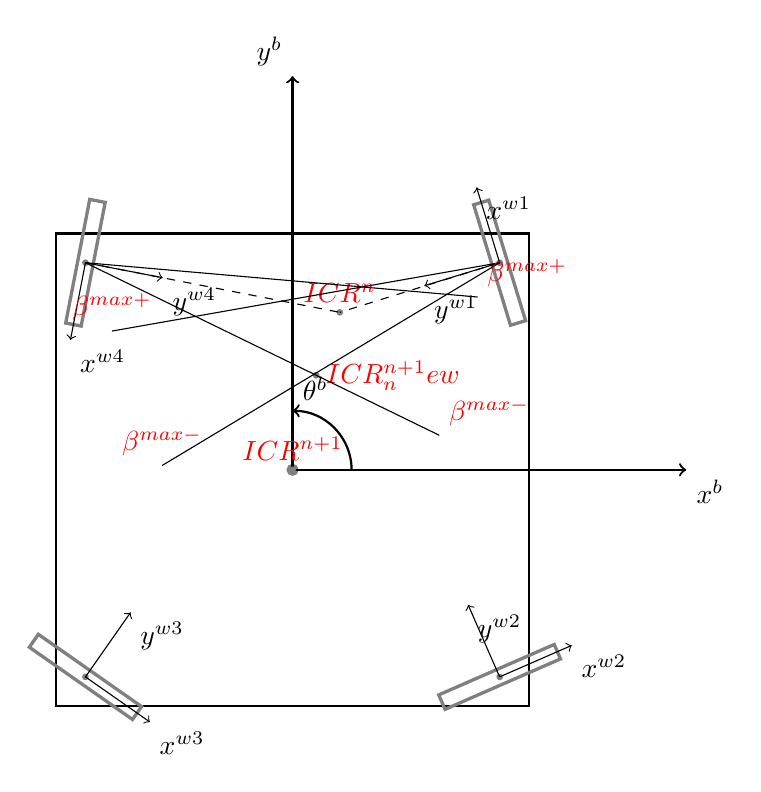
\begin{tikzpicture}
			\pic at(0,0) {platform};
			\pic[rotate=107] at(2.63,2.63) {wheelFrame={1}};
			\pic[rotate=23.6] at(2.63,-2.63) {wheelFrame={2}};
			\pic[rotate=-101] at(-2.63,2.63) {wheelFrame={4}};
			\pic[rotate=-35] at(-2.63,-2.63) {wheelFrame={3}};		
			\filldraw [gray] (0.6,2) circle (1pt) node[above,text=red]{$ICR^n$};
			\filldraw [gray] (0,0) circle (1pt) node[above,text=red]{$ICR^{n+1}$};
			\filldraw [gray] (0.3,1.2) circle (1pt) node[anchor=west,text=red]{$ICR^{n+1}_new$};
			%\draw [rotate=-90, thick, ->] (0,0) -- (1.4,3.3) node[above,text=red]{$\dot{\xi}^{ref}$};
			\draw[dashed] (2.63,2.63)  -- (0.6,2);
			\draw (2.63,2.63)  -- +(190:5) node[above,text=red]{$\beta^{max+}$};
			\draw (2.63,2.63)  -- +(211:5) node[above,text=red]{$\beta^{max-}$};
			%\draw (2.63,-2.63)  -- +(101.2:8);
			%\draw (-2.63,-2.63) -- +(57:9);
			\draw[dashed] (-2.63,2.63)  -- (0.6,2);
			\draw (-2.63,2.63)  -- +(-5:5)node[anchor=south west,text=red]{$\beta^{max+}$};
			\draw (-2.63,2.63)  -- +(-26:5)node[anchor=south west,text=red]{$\beta^{max-}$};
	\end{tikzpicture}
	}
	\caption{try to execute $\dot{\xi}=[0,0,1]$}
	\label{}
\end{figure}
\end{frame}

%%%%%%%%%%%%%%%%%%%%%%%%%%%%%%%%%%%%%%%%%%%%%%%%%%%%%%%%%%%%%%%%%

\begin{frame}{ICR optimization method}
     \begin{figure}
	\centering
	\resizebox{6cm}{!}
      {
	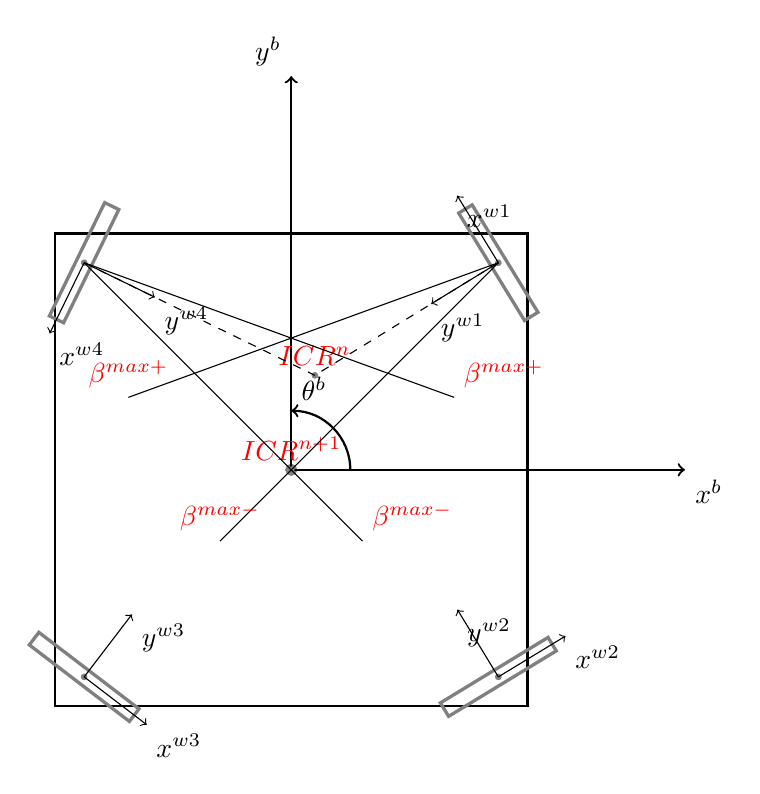
\begin{tikzpicture}
			\pic at(0,0) {platform};
			\pic[rotate=121.5] at(2.63,2.63) {wheelFrame={1}};
			\pic[rotate=31.3] at(2.63,-2.63) {wheelFrame={2}};
			\pic[rotate=-116] at(-2.63,2.63) {wheelFrame={4}};
			\pic[rotate=-37.4] at(-2.63,-2.63) {wheelFrame={3}};		
			\filldraw [gray] (0.3,1.2) circle (1pt) node[above,text=red]{$ICR^n$};
			\filldraw [gray] (0,0) circle (1pt) node[above,text=red]{$ICR^{n+1}$};
			%\draw [rotate=-90, thick, ->] (0,0) -- (1.4,3.3) node[above,text=red]{$\dot{\xi}^{ref}$};
			\draw[dashed] (2.63,2.63)  -- (0.3,1.2);
			\draw (2.63,2.63)  -- +(200:5) node[above,text=red]{$\beta^{max+}$};
			\draw (2.63,2.63)  -- +(225:5) node[above,text=red]{$\beta^{max-}$};
			%\draw (2.63,-2.63)  -- +(101.2:8);
			%\draw (-2.63,-2.63) -- +(57:9);
			\draw[dashed] (-2.63,2.63)  -- (0.3,1.2);
			\draw (-2.63,2.63)  -- +(-20:5)node[anchor=south west,text=red]{$\beta^{max+}$};
			\draw (-2.63,2.63)  -- +(-45:5)node[anchor=south west,text=red]{$\beta^{max-}$};
	\end{tikzpicture}
	}
	\caption{try to execute $\dot{\xi}=[0,0,1]$}
	\label{}
\end{figure}
\end{frame}
%%%%%%%%%%%%%%%%%%%%%%%%%%%%%%%%%%%%%%%%%%%%%%%%%%%%%%%%%%%%%%%%%

\begin{frame}{ICR optimization method}
    With the optimized ICR, we calculate a feasible task space command $\dot{\xi}^{n+1}_{new}$ and execute it.
    \metroset{block=fill}
    \begin{block}{Limitation}
      ICR undefined for pure translation ($\dot{\theta}=0$): representation singularity
    \end{block}
\end{frame}
%%%%%%%%%%%%%%%%%%%%%%%%%%%%%%%%%%%%%%%%%%%%%%%%%%%%%%%%%%%%%%%%%
\begin{frame}{A switching controller}
    So far we have 2 solutions
    \begin{itemize}
        \item Approximation based inverse kinematic control
        \item ICR optimization control
    \end{itemize}
    Both of them have limitations, but they perfectly complement each other.
    \begin{columns}
      \column{0.5\textwidth}
      \metroset{block=fill}
      \begin{block}{ICR far away}
      ICR optimization method fail. But approximation method is accurate.  
      \end{block}
      
      \column{0.5\textwidth}
      \metroset{block=fill}
      \begin{block}{ICR close to platform}
        Approximation method has large error. But ICR optimization mehtod works fine.
      \end{block}
    \end{columns}
    
\end{frame}

%%%%%%%%%%%%%%%%%%%%%%%%%%%%%%%%%%%%%%%%%%%%%%%%%%%%%%%%%%%%%%%%%
\begin{frame}{A switching controller}
The final controller we use has a switching mechanism. Estimate the current ICR from sensor feed back. If it's close to the platform (norm(ICR)<threshold) enable ICR optimization method. Otherwise enable Approximation based inverse kinematic method

\tikzstyle{myarrow}=[->, thick]
\tikzstyle{line}=[-, thick]
    \begin{figure}[t]\label{fig:controller}
	\begin{center}
		\begin{tikzpicture}[scale=0.7]

			
		  %  \node (FKAM) at (-2, 0) [rectangle, draw=blue!50, text=blue!70] {FK};
		    \node (switch) at (2, 0) [diamond, draw=red!50, text=red!70] {switch};
		    \node (ICR) at (2, 2) [rectangle, draw=blue!50, text=blue!70] {ICR optimization};
		    \node (IKAM) at (2, -2) [rectangle, draw=red!50, text=red!70] {Approximation};
			
			\draw[myarrow] (-4, 2) |-(ICR.west) node [anchor=south east]{sensor feedback $\hat{\dot{\beta}},\hat{\beta},\hat{\dot{\phi}}$};
			
			\draw[myarrow] (-4, -2) |-(IKAM.west) node [anchor=south east]{command $\dot{\xi}^{n+1},\ddot{\xi}^{n+1}$};
			\draw[myarrow] (-4, 2) |-(ICR.west) node [anchor=north east]{command $\dot{\xi}^{n+1},\ddot{\xi}^{n+1}$};
% 			\draw[myarrow] (-4,0) --(switch.west) node [anchor=south east]{$\hat{\dot{\xi}},\hat{\ddot{\xi}}$};
            \draw[myarrow] (-4,0) --(switch.west) node [anchor=north east]{sensor feedback $\hat{\dot{\beta}},\hat{\beta},\hat{\dot{\phi}}$};
            \draw[myarrow] (switch.north) -- (ICR.south) node [anchor=north west]{enable};
            \draw[myarrow] (switch.south) --(IKAM.north) node [anchor=south west]{enable};
            \draw[myarrow] (ICR.east) -- +(1,0) node [anchor=north west]{$\dot{\xi}^{n+1}_{new}$};
            \draw[myarrow] (IKAM.east) -- +(1,0) node [anchor=north west]{$\dot{\xi}^{n+1}_{new}$};
		\end{tikzpicture}
	\end{center}
	\caption{Low-level controller structure}
\end{figure}
\end{frame}

%%%%%%%%%%%%%%%%%%%%%%%%%%%%%%%%%%%%%%%%%%%%%%%%%%%%%%%%%%%%%%%%%


%%%%%%%%%%%%%%%%%%%%%%%%%%%%%%%%%%%%%%%%%%%%%%%%%%%%%%%%%%%%%%%%%

\begin{frame}{Experiment}
  3 trajectory is tested each corresponding an inconsistency situation.\\
  Checkout the demo video
  \begin{itemize}
      \item 90 degree turn 
      \item pure rotation
      \item A mixture trajectory
  \end{itemize}
\end{frame}

  
\begin{frame}[standout]
  Questions?
\end{frame}
%%%%%%%%%%%%%%%%%%%%%%%%%%%%%%%%%%%%%%%%%%%%%%%%%%%%%%%%%%%%%%%%%
\appendix

\begin{frame}[fragile]{Backup slides}
  \begin{figure}[!h]
    \centering
    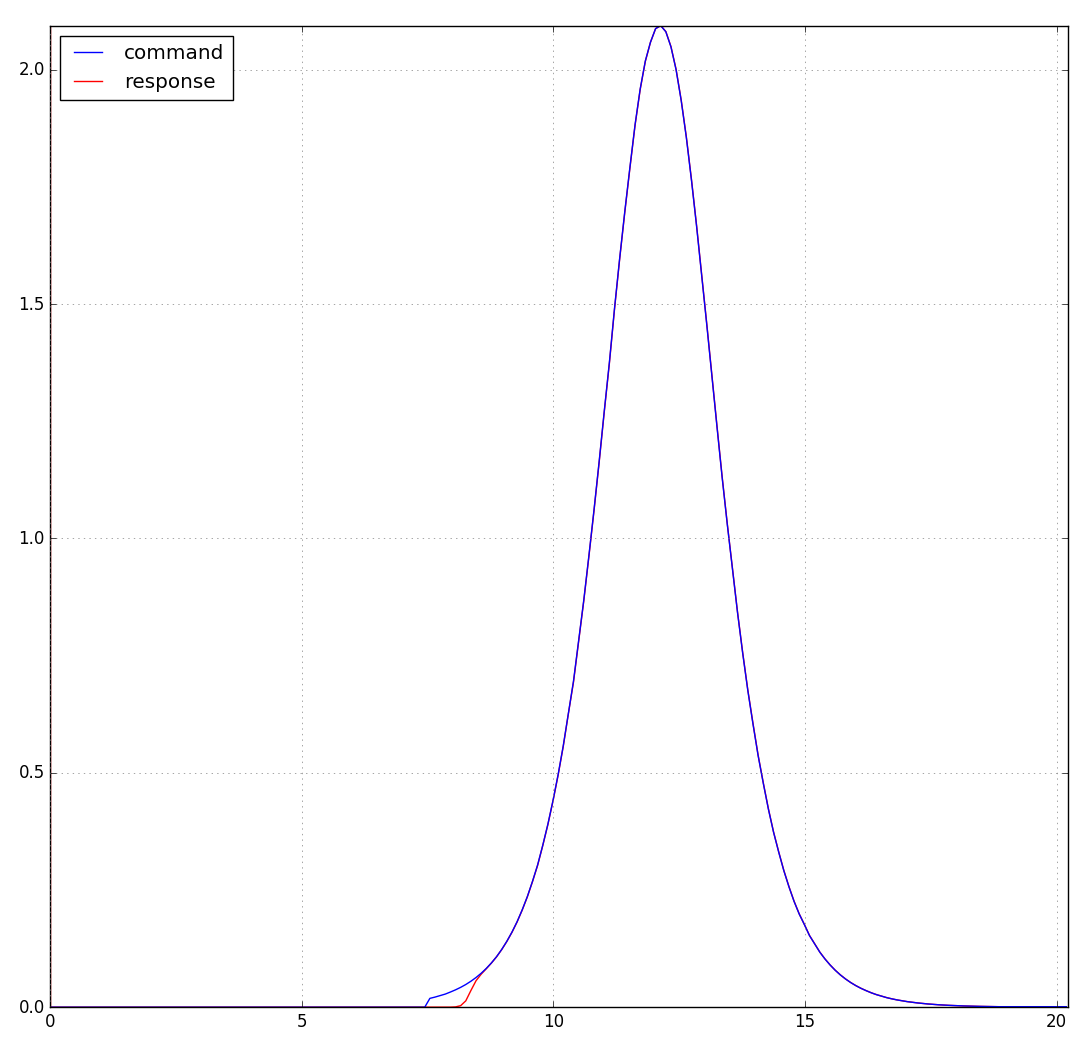
\includegraphics[width=0.7\textwidth]{Figure/PR_t.png}  
    \caption{Reference command and response on $\dot{\theta}$}
    \label{fig:PR_t}
\end{figure}
\end{frame}

%%%%%%%%%%%%%%%%%%%%%%%%%%%%%%%%%%%%%%%%%%%%%%%%%%%%%%%%%%%%%%%%%

\begin{frame}{Figures}
    \begin{figure}
     \centering
     \begin{subfigure}[b]{0.49\textwidth}
         \centering
          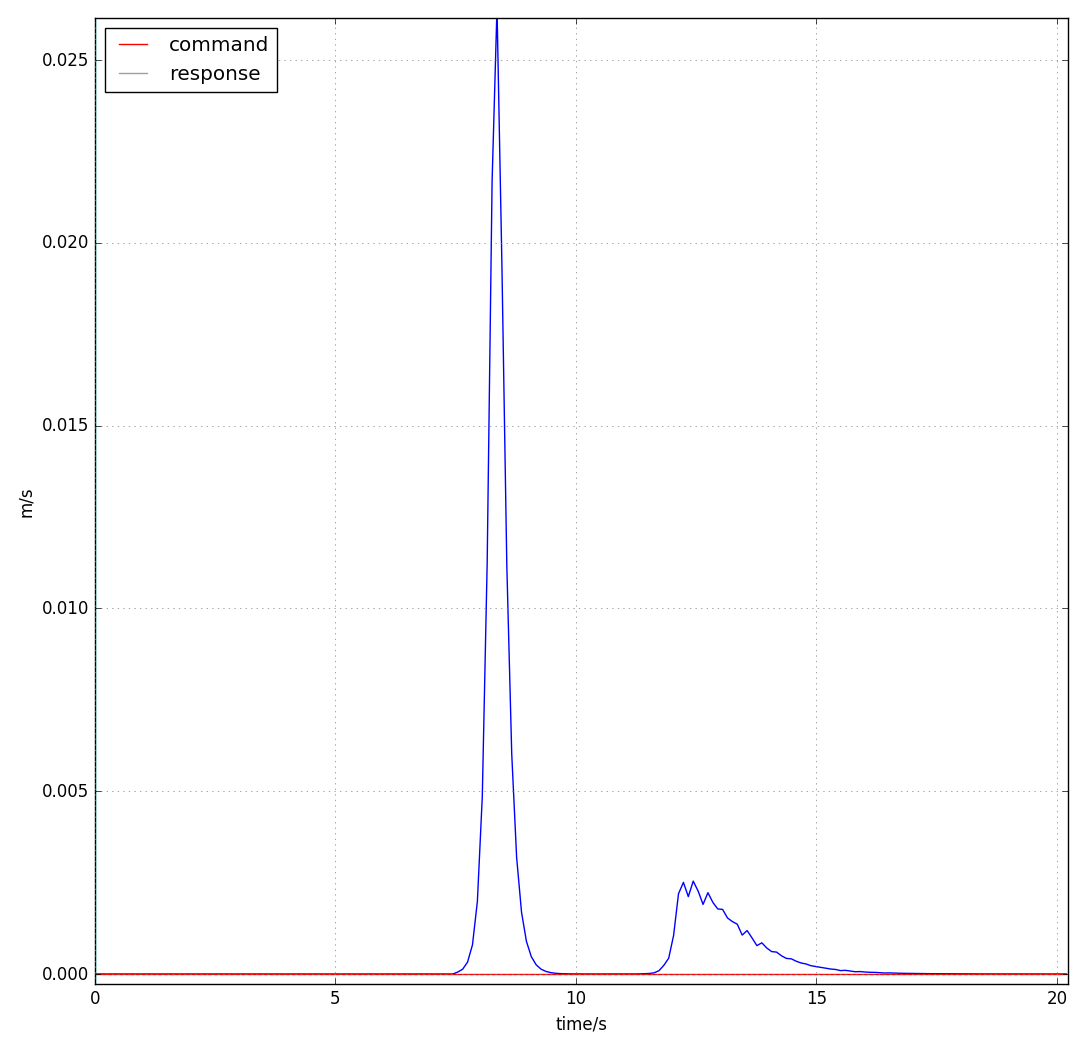
\includegraphics[width=1.2\textwidth]{Figure/PR_x.png}
         \caption{$\dot{x}$}
         \label{fig:PRtranslationX}
     \end{subfigure}
     \hfill
     \begin{subfigure}[b]{0.49\textwidth}
         \centering
         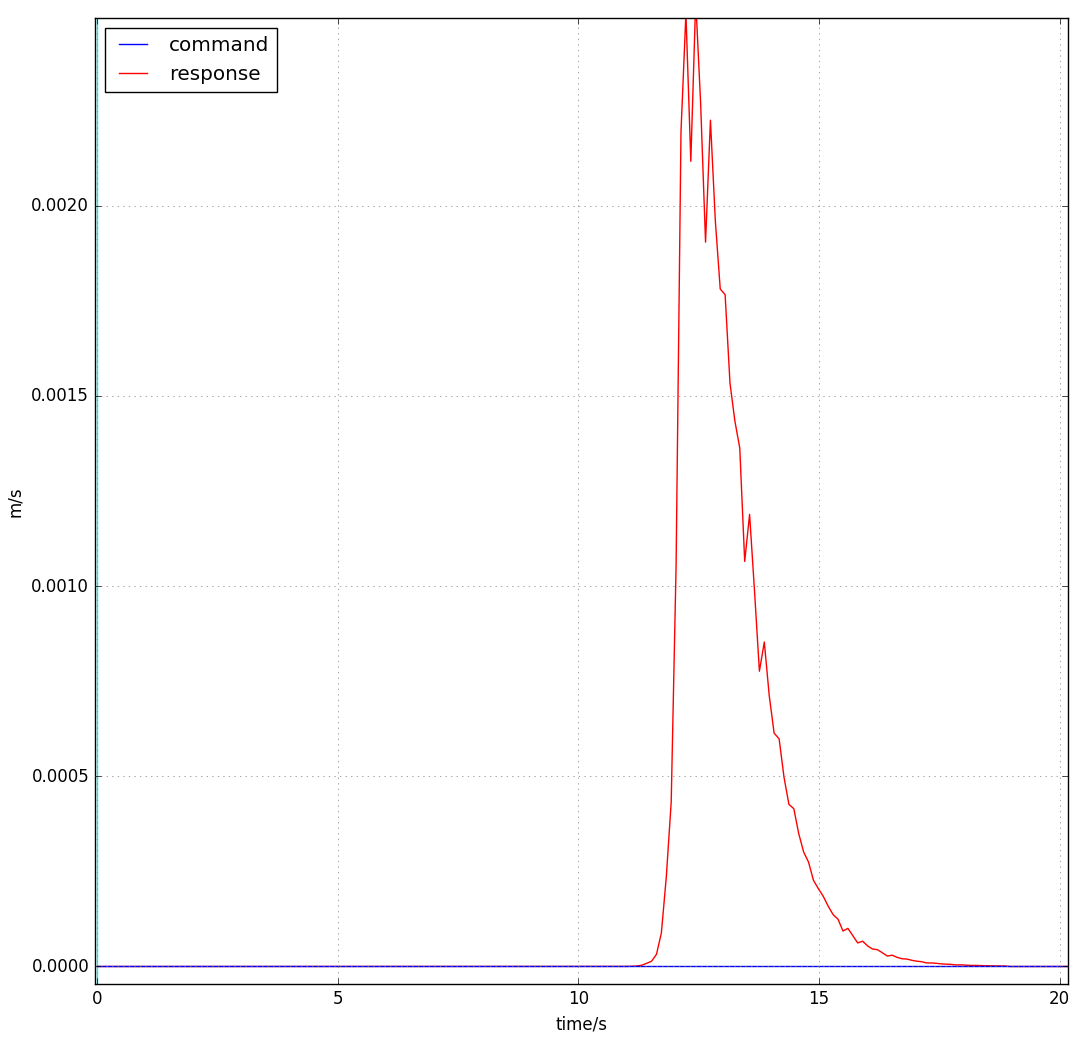
\includegraphics[width=1.2\textwidth]{Figure/PR_y.png}
         \caption{$\dot{y}$}
         \label{fig:PRtranslationY}
     \end{subfigure}
     
        \caption{translation velocity}
        \label{fig:PRtranslation}
\end{figure}
\end{frame}
%%%%%%%%%%%%%%%%%%%%%%%%%%%%%%%%%%%%%%%%%%%%%%%%%%%%%%%%%%%%%%%%%
\begin{frame}{Figures}
\begin{figure}[!h]
    \centering
    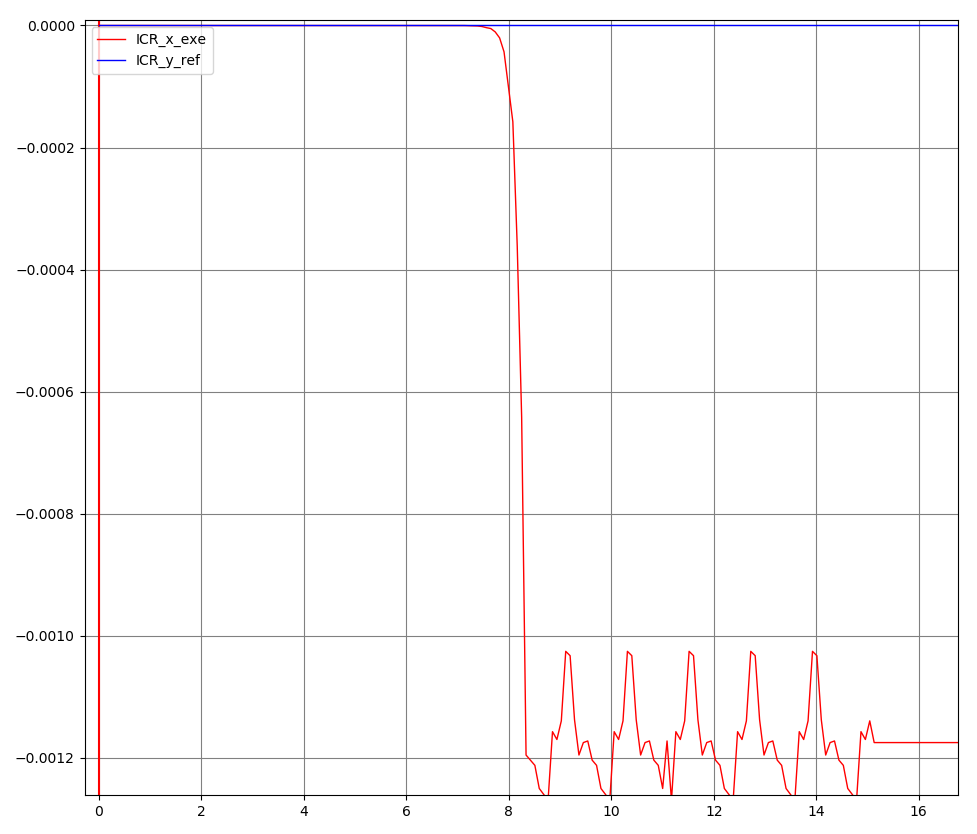
\includegraphics[width=0.7\textwidth]{Figure/PR_ICR_x.png}
    \caption{$\Tilde{ICR_x}$ }
    \label{fig:PR_ICRx}
\end{figure}
\end{frame}
%%%%%%%%%%%%%%%%%%%%%%%%%%%%%%%%%%%%%%%%%%%%%%%%%%%%%%%%%%%%%%%%%
\begin{frame}{Figures}
    
\begin{figure}[!h]
    \centering
    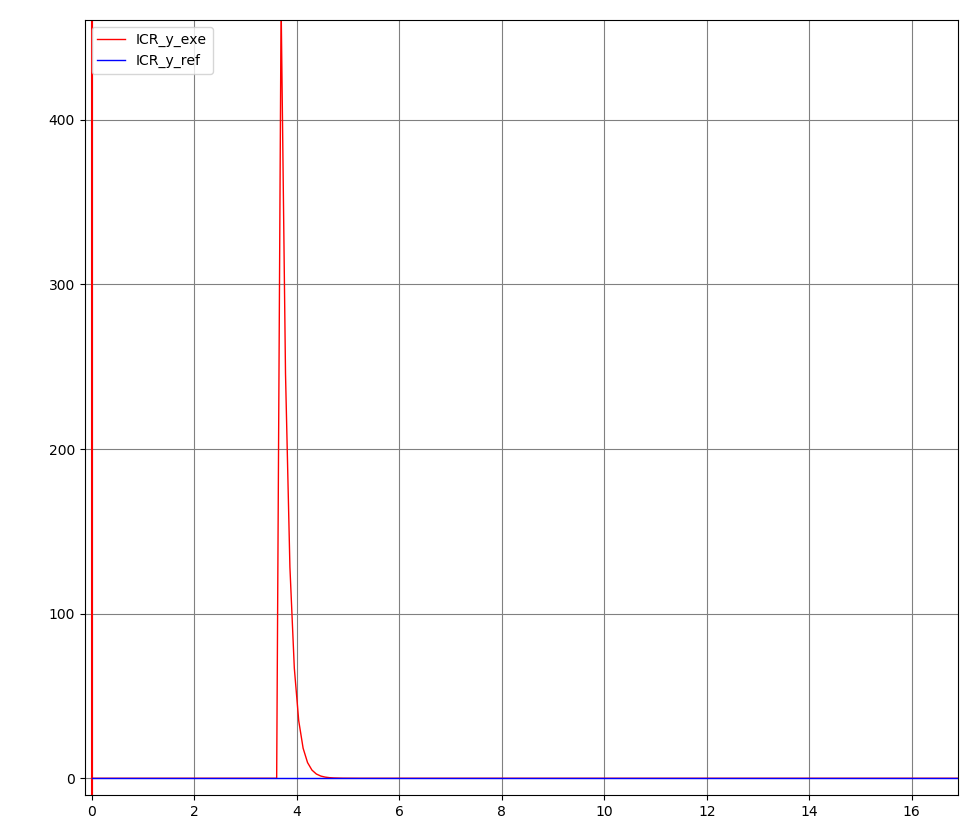
\includegraphics[width=0.7\textwidth]{Figure/PR_ICR_y.png}
    \caption{$\Tilde{ICR_y}$ }
    \label{fig:PR_ICRy}
\end{figure}
\end{frame}
%%%%%%%%%%%%%%%%%%%%%%%%%%%%%%%%%%%%%%%%%%%%%%%%%%%%%%%%%%%%%%%%%


\end{document}
